\documentclass[12pt]{article}

\usepackage[margin=50pt]{geometry}
\usepackage{amsmath}
\usepackage{amsfonts}
\usepackage{amssymb}
\usepackage{graphicx}
\usepackage{subcaption}

\graphicspath{/images}
\geometry{footskip=0.8cm}

\title{Theoretical Computer Science}
\author{Thomas Vroom}

\begin{document}
\maketitle

%
% Lecture 1
%
\section*{Lecture 1 - Strings and Languages}
Computer science (sometimes called \textbf{computation science}) is the study of processes that interact with data and that can be represented as data in the form of programs.
It enables the use of \textbf{algorithms} to manipulate, store and communicate digital information.
A computer scientist studies the \textbf{theory of computation} and the practise of designing software systems.

\noindent
\\
Theoretical computer science is a \textbf{mathematical} study of computation.

\begin{itemize}
    \item \textbf{Computability Theory:} is there a finite algorithm to solve the problem?
    \item \textbf{Computational Complexity Theory:} is there a \textit{good} algorithm for the problem?
\end{itemize}

\subsection*{Alphabets}
An \textbf{alphabet} is a finite set of symbols (e.g. $\{ 0, 1 \}$, $\{ a, b, c \}$, ...).
The most common alphabet we will use is the \textbf{binary alphabet} $\{ 0, 1 \}$, but in principle any finite set of objects can be used as an alphabet.

\subsection*{Strings}
A \textbf{string} is a finite sequence of symbols from an alphabet.
For example, $0010$, $1010$, $1101$ are all strings from the binary alphabet $\{ 0, 1 \}$.
A string might contain no symbols at all, this is called the empty string $\epsilon$.

\noindent
\\
Given an alphabet $\Sigma$, we denote by $\Sigma^*$ the set of all strings that we can construct using symbols from $\Sigma$ (\textbf{including} the empty string $\epsilon$).
Given an alphabet $\Sigma$ and an arbitrary string $w$, we say that $w \in \Sigma^*$ if the string $w$ consists of symbols from $\Sigma$.
We assume that the symbol $w$ is not a part of $\Sigma$ to avoid confussion.

\noindent
\\
The \textbf{length} of a string $w$ is denoted by $|w|$ and is the number of characters in $w$.
For example, $|0010| = 4$, $|\epsilon| = 0$.
The $j$th index of a string $w$ is denoted by $w(j)$, where $1 \leq j \leq |w|$.
\textbf{This is not 0-indexed!}
For example, $w = \{ 12345 \}$, $w(1) = 1$, $w(2) = 2$, $w(|w|) = 5$.
$w(0)$ and $\epsilon(j)$ are not valid expressions.

\newpage
\noindent
A \textbf{concatenation} of two strings is a combination of both strings.
For example, if $x = \{ rain \}$ and $y = \{ coat \}$, then the concatenation $xy = \{ raincoat \}$.
This is often also denoted as $x \circ y$.
Note that concatenation is \textbf{associative} ($(uv)w = u(vw)$), but it is not \textbf{commutative} ($xy \neq yx$, unless $x = y$, $x = \epsilon$ or $y = \epsilon$).

\noindent
\\
A string $x$ is a substring of $y$ if there exists strings $u$ and $w$ such that $y = uxw$.
Both $u$ and $w$ can be the empty string $\epsilon$.
Each string is a substring of itself, and $\epsilon$ is a substring of every string.
If $u = \epsilon$, then $x$ is a \textbf{prefix} of $y$.
If $w = \epsilon$, then $x$ is a \textbf{suffix} of $y$.

\noindent
\\
The \textbf{reverse} of a string is denoted by $w^R$.
For example $computer^R$ = $retupmoc$. 

\noindent
\\
Let $w$ be a string over some alphabet $\Sigma$.
We define string $w^i$ for some integer $\geq 0$ as:

\[ w^0 = \epsilon \]

\[ w^i = w \circ w^{i - 1} \]

\noindent
For example, $cat^3$ = $catcatcat$.

\subsection*{Languages}
Let $\Sigma$ be any alphabet.
Any subset of $\Sigma^*$ is called a \textbf{language} (any set of strings).
$\Sigma^*$ itself is also a language; the set of every possible strings that can be constructed with symbols from $\Sigma$ (including $\epsilon$).
$\Sigma$ is also a language; all strings that correspond with symbols of $\Sigma$.
$\varnothing$ is also a language; it includes no strings at all.

\noindent
\\
Languages can be \textbf{finite} of \textbf{infinite}.
Finite languages can be represented by listing all their elements, infinite languages are often represented as:

\[ L = \{ w \in \Sigma^* : \text{ some property of string } w \} \]

\noindent
Since languages are sets, we can use any set-operation on them (union, intersection, etc.).
The complement is often denoted by $\bar{L}$ for simplicity.

\noindent
\\
Given two languages $L_1$ and $L_2$, the \textbf{concatenation} of $L_1$ and $L_2$ (denoted by $L_1 L_2$ or $L_1 \circ L_2$) is defined by:

\[ L_1 L_2 = \{ xy : x \in L_1 \text{ and } y \in L_2 \} \]

\noindent
For example, given languages $A = \{ wolf, tiger \}$ and $B = \{ dog, cat \}$, the concatenation is $AB = \{ wolfdog, wolfcat, tigerdog, tigercat \}$.

\noindent
\\
In the same way, we define language $L^i$ for any integer $\geq 0$ as:

\[ L^0 = \{ \epsilon \} \]

\[ L^i = L \circ L^{i - 1} \]

\newpage
\subsection*{Kleene Star}
For some language $L$, $L^*$ is the set we get by concatenating 0, 1, 2 or more strings from $L$:

\[ L^* = L^0 \cup L^1 \cup L^2 \cup ... \cup L^k  \]

\noindent
For all $k \geq 0$.

\noindent
\\
For example, let $L = \{ a, b, c \}$ ($L$ is a language, not an alphabet, it just happens all strings in $L$ have length 1):

\[ L^* = \{ \epsilon, a, b, aa, bb, cc, ab, ba, bc, cb, ac, ca, abc, acb, acba, ... \} \]

%
% Lecture 2
%
\section*{Lecture 2 - Regular Expressions}
\subsection*{Language Recognition Problem}
Given $L \subseteq \Sigma^*$ for some alphabet $\Sigma$, and given some string $w \in \Sigma^*$, is it true that $w \in L$?
For some $L$ this is easy, for some hard, and for some impossible.

\noindent
\\
For this problem we only care about \textit{finite} languages, as \textit{infinite} languages are impossible to solve.
From $\Sigma^*$ we can create \textbf{countably infinite} many strings (recall that a set is countably infinite if there is a \textbf{bijection} between the natural numbers $\mathbb{N}$ and the elements of the set).
How many subsets of $\Sigma^*$ exist?
This is the \textbf{powerset} of $\Sigma^*$, and is \textbf{uncountably infinite}.
Thus, there are \textbf{countably infinite} possible representations over a finite alphabet, but \textbf{uncountably infinite} possible languages.

\noindent
\\
If a language is finite, we can represent it by listing all its elements (countably infinite).
\textbf{Regular expressions} can be used to represent infinite languages.

\subsection*{Regular Expressions}
Sequences of symbols that tell us how to construct a language using only standard operations ($\circ, *, \cup$).

\noindent
\\
\textit{Example:} Let $\{ L = w \in \{ 0, 1 \}^* : \text{w has 2 or 3 occurances of the symbol 1, but the first and second }$\\$\text{occurance are not consecutive} \}$.
This includes strings like $1001, 101, 101010, 1011$, but not $00110, $\\$1101, 100, 1010101$.
The regular expression of this language works like this:

\noindent
\\
\textit{Put zero or more 0 symbols followed by 1, followed by 1 or more 0 symbols followed by 1, followed by zero or more 0 symbols, possibly followed by 1 and zero or more 0 symbols or nothing:}

\[ 0^*100^*10^*(10^* \cup \varnothing^*) \]

\noindent
Since this expression only contains symbols from the alphabet, concatenation, stars, unions and parenthesis, it is called a \textbf{regular expression}.
Recall that $\varnothing^* = \epsilon$.

\noindent
\\
For a regular expression $R$, $R^*$ means any number of concatenations of strings that can be constructed from $R$.
Since there might be multiple regular expressions describing the same language, we denote by $L(R)$ the language which $R$ describes.
Two regular expressions are equivalent if $L(R_1) = L(R_2)$.

\newpage
\noindent
The \textbf{order of operations} is: $* \rightarrow \circ \rightarrow \cup$.
$(0 \cup 1)$ is the same as $(1 \cup 0)$.
For regular expressions, $(R_1 \circ R_2) \circ R_3 = R_1 \circ (R_2 \circ R_3) = R_1 \circ R_2 \circ R_3$ (same for union).
$R \circ \varnothing = \varnothing$ and $R \cup \varnothing = R$.

\noindent
\\
More examples:
\begin{itemize}
    \item $(0 \cup 1)0(0 \cup 1)$ describes the language of all strings of length 3 whose middle symbol is 0.
    \item $(0 \cup 1)^*$ all strings made out of 0 and 1 symbols (and $\epsilon$).
    \item $(0^* \cup 1^*)$ all strings made out of only 0 or only 1 symbols (and $\epsilon$).
    \item $(0^*1^*)$ all strings with zero or more 0 symbols, followed by zero or more 1 symbols.
    \item $(0 \cup 1)^*1$ all strings that end in 1.
    \item $(0 \cup 1)^*101(0 \cup 1)^*010(0 \cup 1)^*$ all strings that include the substrings $101$ and $010$ in that order.
\end{itemize}

\subsection*{Regular Languages}
A language $L$ over some alphabet $\Sigma$ is called \textbf{regular} if there exists some regular expression $R$ that describes $L$.
If languages $L_1$ and $L_2$ are regular languages, then $L_1 \cup L_2$, $L_1 L_2$, $L_1^*$ are also regular languages.
Every finite language is automatically a regular language (they can be described as the union of all their elements).

\noindent
\\
In order to show that a language $L$ is described by a regular expression $R$, we need to show that:
\begin{itemize}
    \item Every string of $L$ is described by $R$.
    \item Every string produced by $R$ belongs to $L$.
\end{itemize}

\noindent
Tips for finding regular expressions for languages:
\begin{itemize}
    \item Consider a 'typical' string from $L$ (write out multiple).
    \item Look at the structure of the strings with the language description in consideration.
\end{itemize}

\noindent
If the description contains a negation, rewrite it to an \textbf{equivalent affirmative} description.\\
\textit{For example:} $w$ does not start with a 1 $\Leftrightarrow$ $w$ starts with a 0, $w$ does not contain substring $011$ $\Leftrightarrow$ every substring $01$ must be followed by a 0, etc.

%
% Lecture 3
%
\newpage
\section*{Lecture 3 - Deterministic Finite Automata}
\subsection*{Finite Automata}
\textbf{Finite Automata} (also known as \textbf{Finite State Machines}) are simple machines that can solve the language recognition problem (decide if some string $w$ belongs to some language $L$).
This machine $M$ either \textit{accepts} or \textit{rejects} language $L$ if provided with string $w$.

\begin{figure}[h]
    \centering
    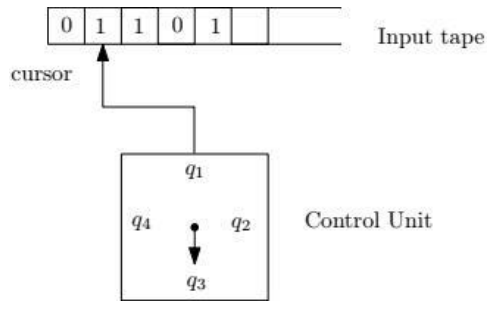
\includegraphics[scale=0.75]{images/finite_automata.PNG}
    \caption{Components of a finite automata.}
\end{figure}

\noindent
A finite automata has the following components:

\begin{itemize}
    \item A \textbf{tape} that extends to infinity. It has \textbf{cells}, each of which holds one \textbf{symbol}.
    \item A \textbf{cursor} that reads one symbol from the tape at a time. It can only move to the right on the tape, and only one symbol at a time.
    \item A \textbf{control unit} that stores the current \textbf{state}. Given the current state and the symbol read by the cursor, it picks a new state.
\end{itemize}

\subsection*{Deterministic Finite Automata}
A deterministic finite automata (DFA) is a five-tuple: $(Q, \Sigma, q_0, \delta, F)$.

\begin{itemize}
    \item $Q$ is a \textit{finite} set of \textbf{states}.
    \item $\Sigma$ is the alphabet of \textbf{input symbols}.
    \item $q_0 \in Q$ is the \textbf{initial state}.
    \item $\delta: Q \times \Sigma \rightarrow Q$ is the \textbf{transition function}.
    \item $F \subseteq Q$ is the set of \textbf{final states}.
\end{itemize}

\newpage
\noindent
\begin{figure}[h]
    \centering
    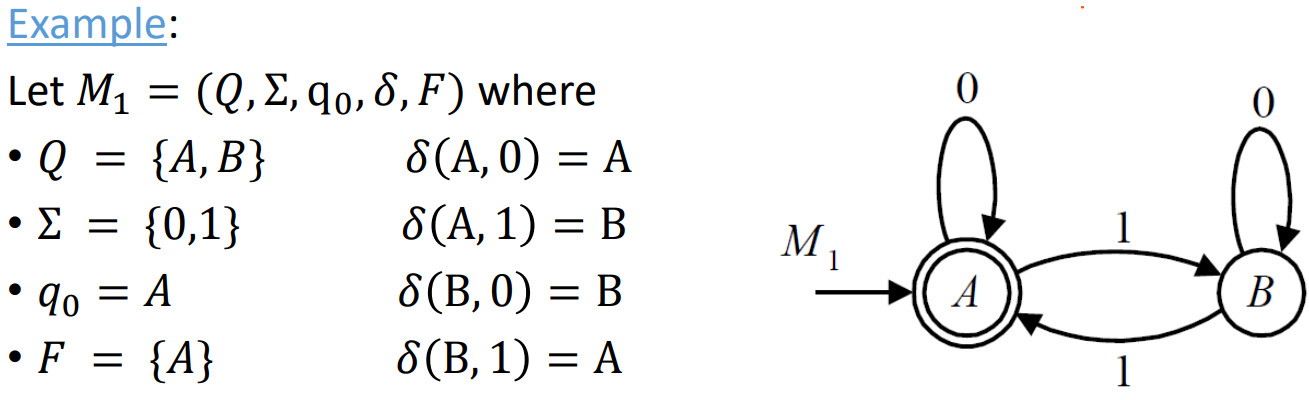
\includegraphics[scale=0.6]{images/dfa_example1.PNG}
    \caption{Note that the incoming arrow represents the initial state, and a circled state represents a final state.}
\end{figure}

\noindent
Every string $w$ has a unique \textit{walk} in the graph of a DFA.
A DFA $M$ \textit{accepts} a string $w$ iff the unique walk of this string ends in a final state.
A DFA $M$ \textit{accepts} a language $L$ iff $M$ accepts all strings in $L$ \textbf{and} \textit{rejects} every other string.

\noindent
\\
If we take the DFA $M$ shown above with string $w = 1001$, we can denote this computation as a sequence of states and remaining characters to be read (this is called the \textbf{configuration}):

\[ (A, \textbf{1}001) \rightarrow (B, \textbf{0}01) \rightarrow (B, \textbf{0}1) \rightarrow (B, \textbf{1}) \rightarrow (A, \epsilon) \]

\noindent
$M$ \textit{accepts} string $w$ if we end up with $\epsilon$ on a final state.
More specifically, we say that DFA $M = (Q, \Sigma, q_0, \delta, F)$ accepts a string $x \in \Sigma^*$ if $(q_0, x) \rightarrow^* (q, \epsilon)$ and $q \in F$.
With $(q_0, x) \rightarrow^* (q, \epsilon)$ we mean that the configuration $(q_0, x)$ can reach the configuration $(q, \epsilon)$ in zero or more steps.

\subsection*{Examples}

\begin{figure}[h]
    \centering
    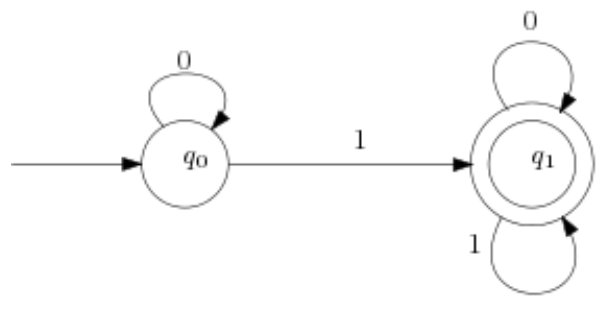
\includegraphics[scale=0.75]{images/dfa_example2.PNG}
    \caption{DFA that recognizes the language of all strings that contain at least one 1.}   
\end{figure}

\newpage
\begin{figure}[h]
    \centering
    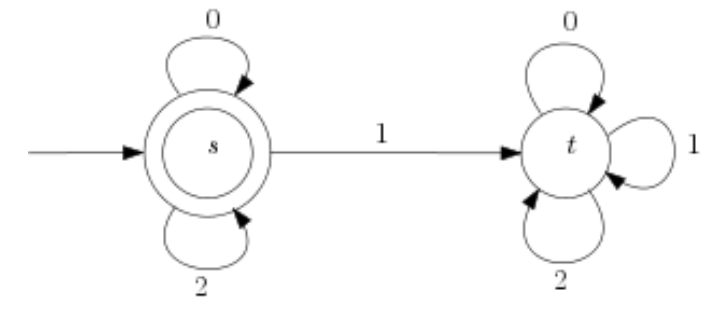
\includegraphics[scale=0.75]{images/dfa_example3.PNG}
    \caption{DFA that recognizes the language of all strings that do not contain a 1.}
\end{figure}

\noindent
Note that state $t$ in the figure above is called a \textbf{sink}.

\begin{figure}[h]
    \centering
    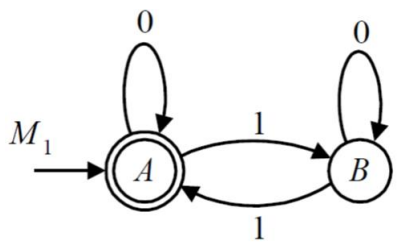
\includegraphics[scale=0.8]{images/dfa_example4.PNG}
    \caption{DFA that recognizes the language of all strings with an even number of 1's.}
\end{figure}

\begin{figure}[h]
    \centering
    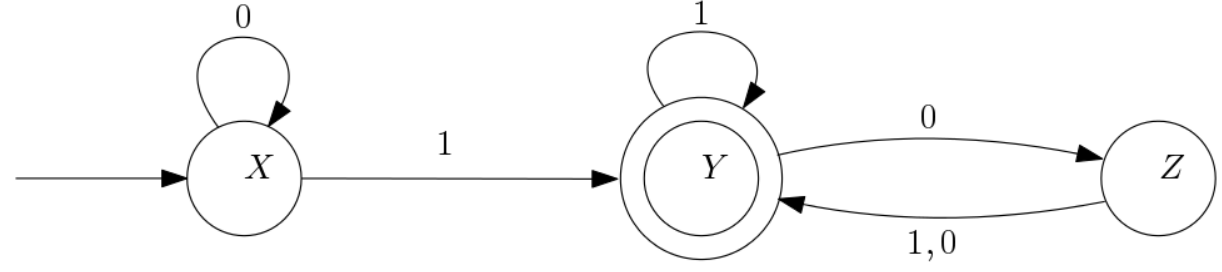
\includegraphics[scale=0.5]{images/dfa_example5.PNG}
    \caption{DFA that recognizes the language of all strings that end with a 1 or an even number of 0's.}
\end{figure}

\begin{figure}[h!]
    \centering
    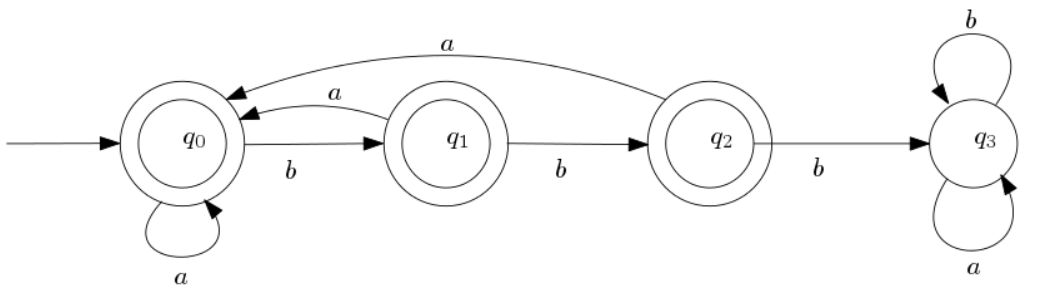
\includegraphics[scale=0.55]{images/dfa_example6.PNG}
    \caption{DFA that recognizes the language of all strings that do not contains 3 consecutive b's.}
\end{figure}

%
% Lecture 4
%
\newpage
\section*{Lecture 4 - Non-Deterministic Finite Automata}

\begin{figure}[h]
    \centering
    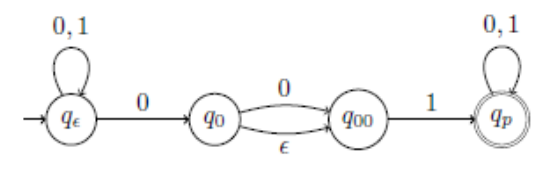
\includegraphics{images/nfa_example1.PNG}
    \caption{NFA describing the language $(0 \cup 1)^* (001 \cup 01) (0 \cup 1)^*$.}
\end{figure}

\noindent
Differences:

\begin{itemize}
    \item From some states, we can reach \textbf{multiple states} with one symbol.
    \item Some states have \textbf{no transitions} for some symbols.
    \item $\epsilon$-transitions can reach some states \textbf{without needing a symbol}.
\end{itemize}

\noindent
Given the string $w = 001$ on the above example, we can reach states $\{ q_{\epsilon}, q_0, q_{00}, q_p \}$.

\noindent
\\
An NFA \textit{accepts} a string $w$ iff a final state \underline{can} be reached starting from the initial state.
A non-deterministic finite automata (NFA) is a five-tuple: $(Q, \Sigma, q_0, \Delta, F)$.

\begin{itemize}
    \item $Q$ is a \textit{finite} set of \textbf{states}.
    \item $\Sigma$ is the alphabet of \textbf{input symbols}.
    \item $q_0 \in Q$ is the \textbf{initial state}.
    \item $\Delta: Q \times \{\Sigma \cup \{\epsilon\}\} \rightarrow P(Q)$ is the \textbf{transition relation}.
    \item $F \subseteq Q$ is the set of \textbf{final states}.
\end{itemize}

\noindent
Similar to DFA's, an NFA accepts a string $w$ if $(q_0, x) \rightarrow^* (q, \epsilon)$ and $q \in F$, but since there are multiple paths possible we only care about if there \textbf{exists} a path for which this property holds.

\begin{figure}[h]
    \centering
    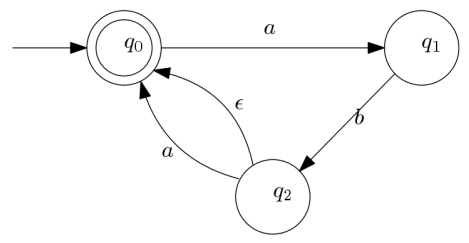
\includegraphics[scale=0.8]{images/nfa_example2.PNG}
    \caption{Example: does this system accept the string $abab$? Yes, because we can take the path $a \rightarrow b \rightarrow \epsilon \rightarrow a \rightarrow b \rightarrow \epsilon$, and end on a final state.}
\end{figure}

\newpage
\noindent
Constructing a finite automata that recognizes all string over $\{0, 1\}$ that contain a 1 in the third position from the end:

\begin{figure}[h]
    \centering
    \begin{minipage}{.5\textwidth}
      \centering
      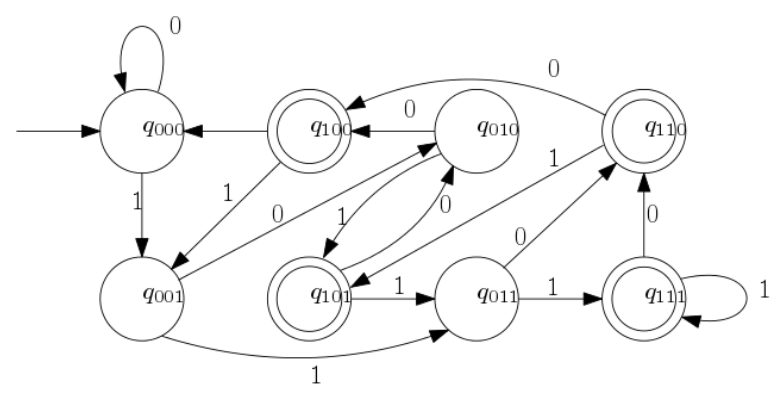
\includegraphics[scale=0.45]{images/nfa_dfa_difference1.PNG}
      \captionof{figure}{DFA}
    \end{minipage}% <- this is necessary
    \begin{minipage}{.5\textwidth}
      \centering
      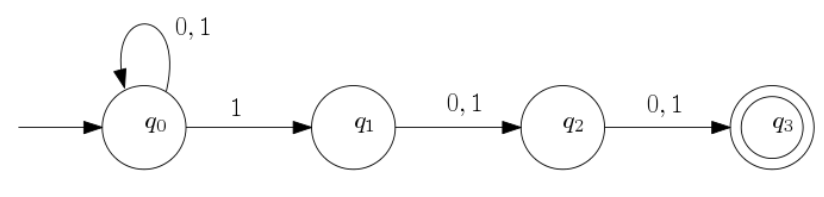
\includegraphics[scale=0.5]{images/nfa_dfa_difference2.PNG}
      \captionof{figure}{NFA}
    \end{minipage}
\end{figure}

\noindent
Some examples:

\begin{figure}[h]
    \centering
    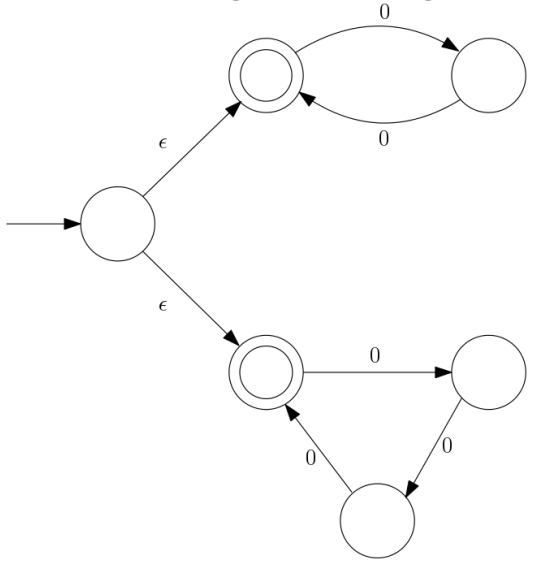
\includegraphics[scale=0.65]{images/nfa_example3.PNG}
    \caption{NFA that recognizes the language of all strings whose length is a multiple of 2 or 3.}
\end{figure}

\begin{figure}[h!]
    \centering
    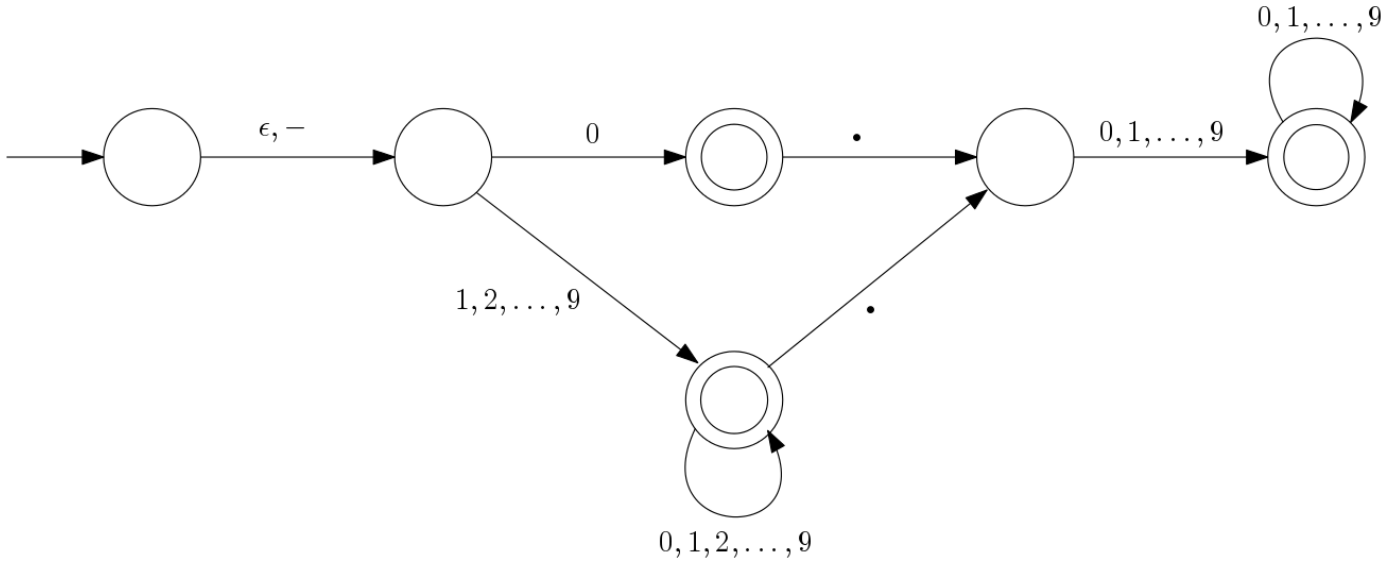
\includegraphics[scale=0.45]{images/nfa_example4.PNG}
    \caption{NFA that recognizes the language of all strings that represent valid decimal numbers.}
\end{figure}

%
% Lecture 5
%
\newpage
\section*{Lecture 5 - Equivalence}
Two finite automata $M_1$ and $M_2$ are equivalent iff $L(M_1) = L(M_2)$ (i.e. they recognize the same language).

\noindent
\\
If we want to construct a DFA from an NFA, we need to keep track of what states can be reached at a certain point in the NFA.
Given $q \in Q$, $E(q)$ represents the set of states $\subseteq Q$ that can be reached from $q$ by taking zero or more $\epsilon$-transitions (also called the \textbf{$\epsilon$-closure}).
Similarly, given $q \in Q$ and $\sigma \in \Sigma$, $R(q, \sigma)$ represents the set of states $\subseteq Q$ that can be reached from $q$ \textbf{after} reading $\sigma$ (including $\epsilon$-transitions afterwards).
This 'set of states' is also called a \textbf{superstate}.

\begin{figure}[h]
    \centering
    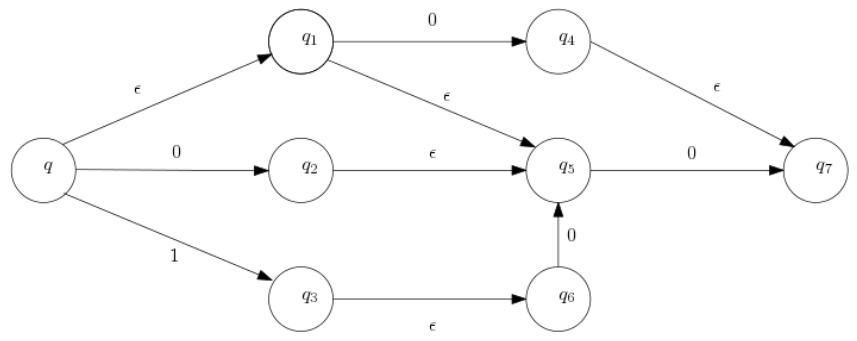
\includegraphics[scale=0.75]{images/nfa_example5.PNG}
    \caption{Example NFA. $E(q) = \{q, q_1, q_5\}$, $R(q, 0) = \{q_2, q_5\}$, ...}
\end{figure}

\subsection*{Constructing a DFA from an NFA}
Let $N = (Q, \Sigma, q_0, \Delta, F)$ be a given NFA.
We will construct an \textbf{equivalent} DFA $M = (Q', \Sigma', s, \delta, F')$ where:

\begin{itemize}
    \item $Q' = P(Q) = s^Q$ is the \textbf{powerset} of $Q$ (set of all subsets).
    \item $\Sigma' = \Sigma$.
    \item $s = E(q_0)$.
    \item $F' = \{S \subseteq Q : S \cap F \neq \varnothing\}$ (all sets in $Q'$ that contain at least one final set).
    \item $\delta$ is defined as:
\end{itemize}

\[ \forall (S \subseteq Q \text{ and } \sigma \in \Sigma) \text{ } \delta(S, \sigma) = \bigcup_{q \in S} R(q, \sigma) \]

\[ \text{"for all sets } S \in Q' \text{ and all symbols } \sigma \text{, } \delta(S, \sigma) \text{ equals the union of } R(q, \sigma) \text{ for all states } q \in S \text{".} \]

\newpage
\begin{figure}[h]
    \centering
    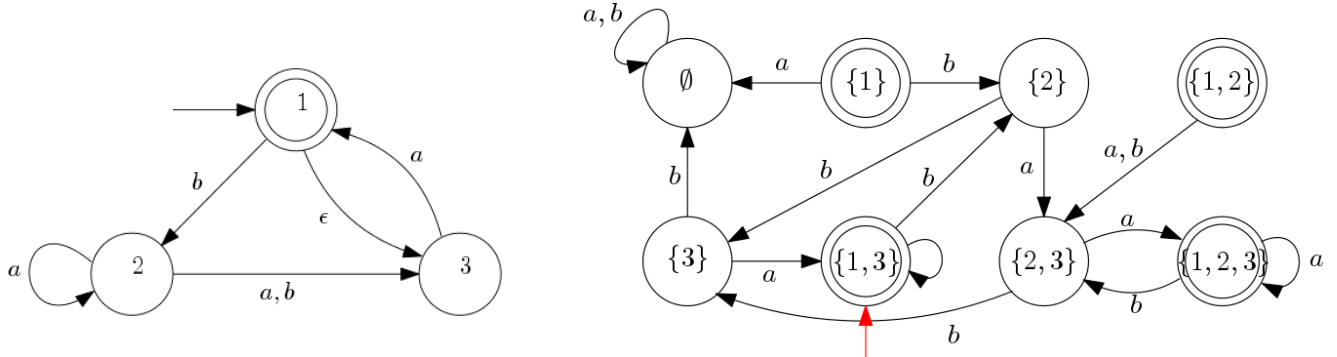
\includegraphics[scale=0.6]{images/dfa_from_nfa.PNG}
    \caption{From NFA (left) to DFA (right).}
\end{figure}

\subsection*{Closure Properties}
\begin{itemize}
    \item \textbf{Union:} let $s_1$ and $s_2$ be the initial states of two seperate FA's. To combine these two FA's define a new initial state $s_n$ and connect this state to both old initial states through an $\epsilon$-transition.
    \item \textbf{Complement:} let $M = \{Q, \Sigma, q_0, \delta, F\}$ be a \textbf{DFA} that recognizes the language $L(M)$. The language $\overline{L(M)}$ is recognized by $\overline{M} = \{Q, \Sigma, q_0, \delta, Q - F\}$. This does \textbf{not} work for NFA's, where $\epsilon$-transitions can cause some strings to be accepted by both machines.
    \item \textbf{Concatenation:} let $f_1, f_2, ... , f_n$ be the final states of an FA and $s_1$ be the initial state of another FA. To combine these two FA's construct $\epsilon$-transitions from $f_1, f_2, ... , f_n$ to $s_1$.
    \item \textbf{Kleene-Star:} let $s_1$ be the initial state and $f_1, f_2, ... , f_n$ be the final states of the same FA. To create the Kleene-Star closure of this FA construct $\epsilon$-transitions from $f_1, f_2, ... , f_n$ to $s_1$, and then create a new initial state $s_0$, that is also final, and connect it to $s_1$ through an $\epsilon$-transition.
    \item \textbf{Intersection:} use $A \cap B = \overline{\bar{A} \cup \bar{B}}$.
\end{itemize}

\newpage
\subsection*{Constructing an FA from a Regular Expression}
\textbf{Recursive algorithm:} split the regular expression $R$ into smaller subsections, construct an FA for each of these subsections, then combine these FA's using the closure properties.

\noindent
\\
If $R = a$ for some $a \in \Sigma$, then $L(R) = \{a\}$.
The following NFA recognizes $L(R)$:

\begin{figure}[h]
    \centering
    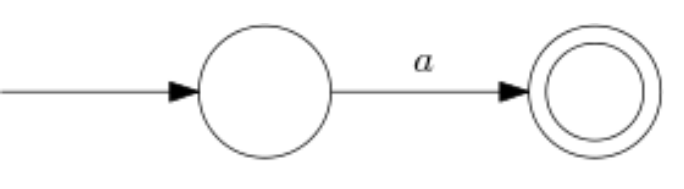
\includegraphics[scale=0.55]{images/thompson1.PNG}
\end{figure}

\noindent
If $R = \epsilon$, then $L(R) = \{\epsilon\}$.
The following NFA recognizes $L(R)$:

\begin{figure}[h]
    \centering
    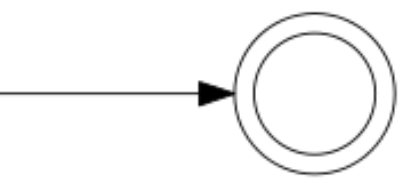
\includegraphics[scale=0.55]{images/thompson2.PNG}
\end{figure}

\noindent
If $R = \varnothing$, then $L(R) = \varnothing$.
The following NFA recognizes $L(R)$:

\begin{figure}[h]
    \centering
    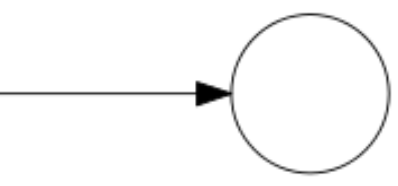
\includegraphics[scale=0.55]{images/thompson3.PNG}
\end{figure}

\begin{figure}[h!]
    \centering
    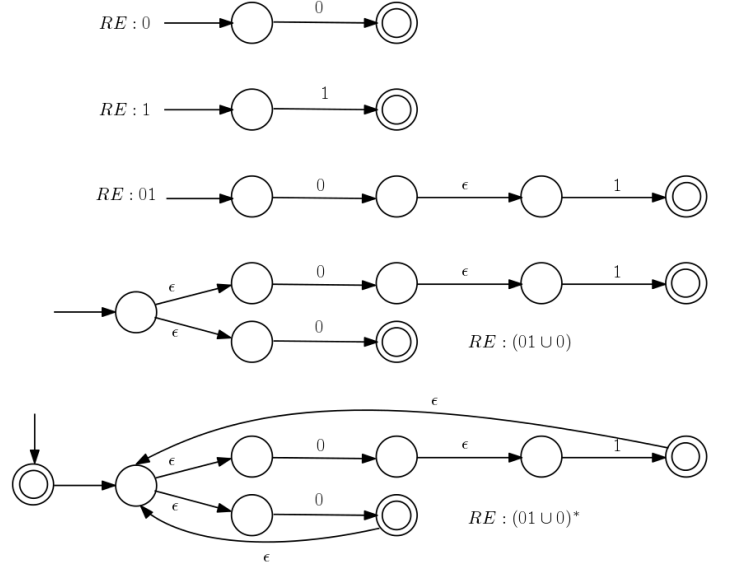
\includegraphics[scale=0.75]{images/retofa_example.PNG}  
    \caption{Example FA that recognizes the regular expression $(01 \cup 0)^*$.}  
\end{figure}

%
% Lecture 6
%
\newpage
\section*{Lecture 6 - Pumping Lemma}
Some languages are \textbf{non-regular}.
E.g. the language $L = \{w = 0^n 1^n : n \geq 0\}$ requires infinite memory to remember the number of leading zeros.
The \textbf{Pumping Lemma} is a way to formally argue about regularity.

\subsection*{The Pumping Lemma for Regular Languages}
($\forall$) For every \textit{infinite} language $L$,\\
($\exists$) there exists an integer $n \geq 1$ such that,\\
($\forall$) for every string $w \in L$ with $|w| \geq n$,\\
($\exists$) there exist strings $x, y, z$ such that $w = xyz$, $|xy| \leq n$, $y \neq \epsilon$\\
($\forall$) and for every integer $i \geq 0$, $xy^iz \in L$.

\noindent
\\
We can use the Pumping Lemma to prove that an \textit{infinite} language $L$ is \textit{non-regular} using a proof by contradiction:

\begin{enumerate}
    \item Assume $L$ is regular, let $n$ be the \textbf{pumping lemma constant} for $L$.
    \item Choose a string $w \in L$ with $|w| \geq n$.
    \item For every way we can break $w$ up into $w = xyz$ with $|xy| \leq n$ and $y \neq \epsilon$,\\find $i \geq 0$ ($i \neq 1$) such that $xy^iz \notin L$.
    \item This contradicts the Pumping Lemma, thus $L$ is not regular.
\end{enumerate}

\noindent
Examples:

\noindent
\\
1) Show that $L = \{w = 0^k 1^k : k \geq 0\}$ is non-regular.
Proof by contradiction:

\begin{enumerate}
    \item Assume $L$ is regular and let $n$ be the pumping lemma constant for $L$.
    \item Take the string $w = 0^n 1^n \in L$ ($|w| \geq n$).
    \item We can describe every way we can break $w$ up into $w = xyz$ with $|xy| \leq n$ and $y \neq \epsilon$ as\\$x = 0^p$, $y = 0^q$, $z = 0^{n - p - q}1^n$ with $p \geq 0$ and $q \geq 1$.
    \item This means we can write $xy^iz$ as $0^p \left(0^q\right)^i 0^{n - p - q} 1^n = 0^{n + (i - 1)q} 1^n$.
    \item For $i = 2$, $xy^2z = 0^{n + q} 1^n$.
    \item $n + q > n$, so $xy^2z = 0^{n + q} 1^n \notin L$, thus $L$ is not regular. $\Box$
\end{enumerate}

\noindent
Note: be careful with you choice of $w$.
If you choose the string $w = 0^s 1^s$ where $s = \frac{n}{2}$ you can't find a contradiction.

\newpage
\noindent
2) Show that $L = \{ww : w \in \{0, 1\}^*\}$ is non-regular.
Proof by contradiction:

\begin{enumerate}
    \item Assume $L$ is regular and let $n$ be the pumping lemma constant for $L$.
    \item Let $w = 0^n 10^n1 \in L$ ($|w| \geq n$).
    \item We can describe every way we can break $w$ up into $w = xyz$ with $|xy| \leq n$ and $y \neq \epsilon$ as\\$x = 0^p$, $y = 0^q$, $z = 0^{n - p - q}10^n1$ with $p \geq 0$ and $q \geq 1$.
    \item For $i = 2$, $xy^2z = 0^{p + 2q}0^{n - p - q}10^n1 = 0^{n + q}10^{n}1$.
    \item $0^{n + q}10^{n}1 \notin L$, thus $L$ is not regular. $\Box$
\end{enumerate}

\noindent
3) Show that $L = \{0^i 1^j : i > j\}$ is non-regular.
Proof by contradiction:

\begin{enumerate}
    \item Assume $L$ is regular and let $n$ be the pumping lemma constant for $L$.
    \item Let $w = 0^{n + 1} 1^n \in L$ ($|w| \geq n$).
    \item We can describe every way we can break $w$ up into $w = xyz$ with $|xy| \leq n$ and $y \neq \epsilon$ as\\$x = 0^p$, $y = 0^q$, $z = 0^{n + 1 - p - q}1^n$ with $p \geq 0$ and $q \geq 1$.
    \item For $i = 0$, $xy^0z = xz = 0^p 0^{n + 1 - p - q} = 0^{n - q + 1}1^n$.
    \item $0^{n - q + 1}1^n \notin L$, thus $L$ is not regular. $\Box$
\end{enumerate}

\noindent
4) Show that $L = \{w \in \{0, 1\}^* : w = w^R\}$ (palindromes) is non-regular.
Proof by contradiction:

\begin{enumerate}
    \item Assume $L$ is regular and let $n$ be the pumping lemma constant for $L$.
    \item Let $w = 0^n10^n$ ($|w| \geq n$).
    \item We can describe every way we can break $w$ up into $w = xyz$ with $|xy| \leq n$ and $y \neq \epsilon$ as\\$x = 0^p$, $y = 0^q$, $z = 0^{n - p - q}10^n$ with $p \geq 0$ and $q \geq 1$.
    \item For $i = 0$, $xy^0z = xz = 0^p0^{n - p - q}10^n = 0^{n - q}10^n$.
    \item $0^{n - q}10^n \notin L$, thus $L$ is not regular. $\Box$
\end{enumerate}

\subsection*{Myhill-Nerode Theorem}
A language $L$ is regular iff \textit{every} set of strings that are pairwise \textbf{distinguishable} by $L$ is \textit{finite}.
Two strings $x, y$ are distinguishable by $L$ if there exists a string $z$ such that exactly one of $xz$ or $yz$ belongs in $L$.
E.g. if $L = \{0^k : k \text{ is even}\}$, then $00$ and $000$ are distinguishable, but $00$ and $0000$ are indistinguishable.

%
% Lecture 7
%
\newpage
\section*{Lecture 7 - Turing Machines}
The main issue with FA's is that we can't use them for languages that require infinite memory, e.g. $L = \{1^n 0^n, n \geq 0\}$.

\subsection*{Pushdown Automata}
A more powerful automata, equipped with a stack.
At each step:

\begin{enumerate}
    \item Read the current symbol $a$ from the input string (left to right).
    \item Read the current symbol $A$ from the top of the stack.
    \item Depending on current state $p$, $a$ and $A$; go to new state $p'$, pop $A$ from the stack and push $B$ to the stack.
\end{enumerate}

\begin{figure}[h]
    \centering
    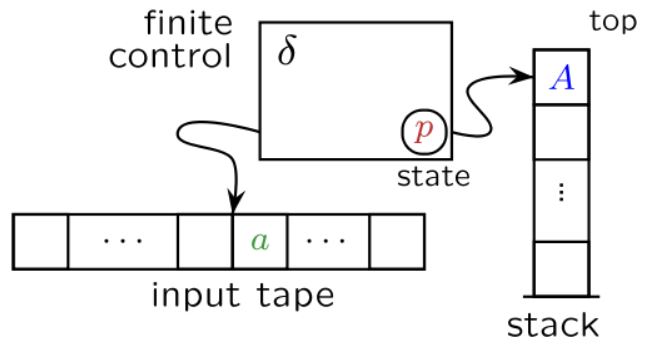
\includegraphics[scale=0.65]{images/pushdownautomata.PNG}
\end{figure}

\noindent
This type of automata can recognize \textbf{context free languages}, this includes $L = \{0^n 1^n, n \geq 0\}$, but also the syntax of every programming language ever created.
There are still some limitations though, for example with only one stack we can't recognize the language $L = \{0^n 1^n 2^n, n \geq 0\}$.

\subsection*{Turing Machines}
Turing machines can define any arbitrary computation (it is the definition of \textit{"what is computable?"}).

\begin{figure}[h!]
    \centering
    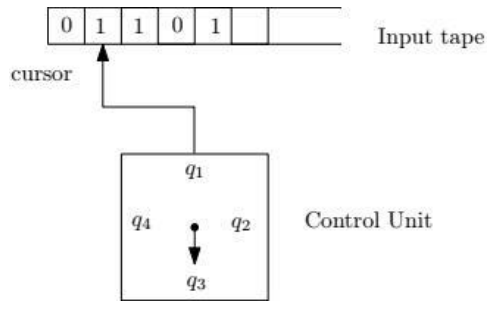
\includegraphics[scale=0.8]{images/finite_automata.PNG}
\end{figure}

\newpage
\noindent
The \textbf{tape} of a Turing machine consists of cells, each one containing a symbol.
There is a leftmost cell $\vartriangleright$, but the tape extends to infinity on the right side.

\noindent
\\
The \textbf{cursor} reads the current cell symbol, but can also \textbf{overwrite} the symbol in the current cell.
The cursor can move one cell to the right, one cell to the left, or stay where it is.

\noindent
\\
A Turing machine $M$ is defined by $M = (Q, \Sigma, \Gamma, \delta, q_0, q_{accept}, q_{reject})$.

\begin{itemize}
    \item $Q$ is a \textbf{finite} set of states (that includes $q_0$, $q_{accept}$, $q_{reject}$, and possibly $q_{halt}$).
    \item $\Sigma$ is the \textit{input} alphabet (any symbols that may be in the input string).
    \item $\Gamma$ is the \textit{tape} alphabet (any symbols that may be on the tape).\\(input alphabet + any auxiliary symbols + \textbf{blank symbol} $\sqcup$).
    \item $\delta$ is the transition function: $Q \times \Gamma \rightarrow Q \times \Gamma \times \{L, R, -\}$.
\end{itemize}

\begin{figure}[h]
    \centering
    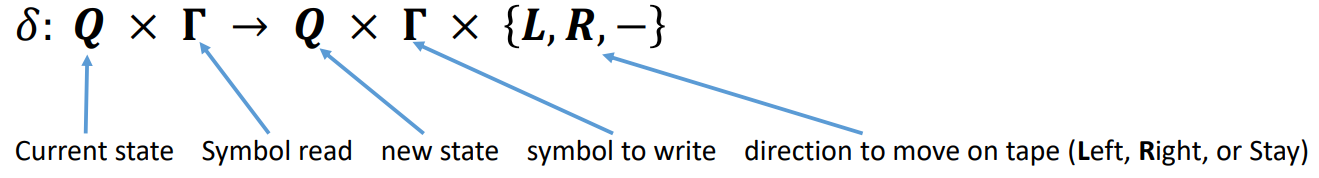
\includegraphics[scale=0.45]{images/turingmachinetransitionfunction.PNG}
\end{figure}

\begin{itemize}
    \item $q_0$ the \textit{starting} state.
    \item $q_{accept}, q_{reject}, q_{halt}$ the \textit{accepting, rejecting, halting} states.
\end{itemize}

\noindent
Since $\delta$ is a function, we are describing \textbf{deterministic} Turing machines.
If $\delta(q_1, a) = (q_2, b, L)$, then from state $q_1$ and by reading symbol $a \in \Gamma$, it replaces $a$ by $b \in \Gamma$, enters states $q_2$ and moves the cursor one cell to the left.
This can be pictured as:

\begin{figure}[h]
    \centering
    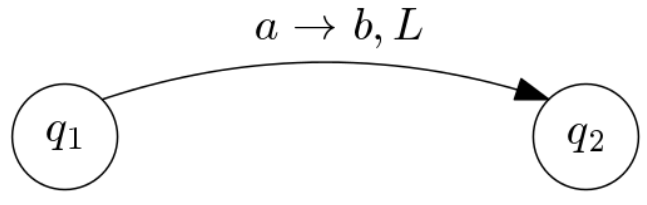
\includegraphics[scale=0.5]{images/turingmachinepicturedtransition.PNG}
\end{figure}

\noindent
The Turing machine always starts in the starting state $q_0$.
The input string has been loaded into the tape, starting from the leftmost cell, and the cursor also starts on the leftmost cell.
For some input string $w \in \Sigma^*$, a Turing machine can eventually:

\begin{itemize}
    \item Enter state $q_{accept}$ (machine terminates and \textbf{accepts} the input string).
    \item Enter state $q_{reject}$ (machine terminates and \textbf{rejects} the input string).
    \item Halt on $q_{halt}$.
    \item Enter an infinite loop (\textbf{deadlock}).
\end{itemize}

\noindent
We assume the cursor cannot move to the left of the leftmost cell of the tape.
If this operation occurs the cursor will stay on the leftmost cell instead.

\newpage
\noindent
For example, $M_1 = (\{q_0, q_{accept}, q_{reject}\}, \{a, b\}, \{a, b, \sqcup\}, \delta, q_0, q_{accept}, q_{reject})$, where $\delta$ equals:

\[ \delta(q_0, a) = (q_0, \sqcup, R) \]
\[ \delta(q_0, b) = (q_0, \sqcup, R) \]
\[ \delta(q_0, \sqcup) = (q_0, \sqcup, R) \]

\noindent
This machine erases all symbols on the type and will infinitely go the right (deadlock).
For $\delta$ equals:

\[ \delta(q_0, a) = (q_0, b, R) \]
\[ \delta(q_0, b) = (q_0, a, R) \]
\[ \delta(q_0, \sqcup) = (q_{accept}, \sqcup, -) \]

\noindent
This machine replaces all $a$ symbols with $b$ symbols (and the other way around), then terminates when it reaches the end of the string.

\noindent
\\
A \textbf{configuration} of a Turing machine is a pair $(q, wau)$, where $q \in Q$ is the current state of the machine, $a \in \Gamma$ is the symbol the cursor is currently pointing at, and $w, u \in \Gamma^*$ is the content to the left / right of the cursor.

\noindent
\\
Let $C_1$ and $C_2$ be two configurations of a Turing machine.
If $C_1$ yields to $C_2$ in one transition, then we can say $C_1 \rightarrow C_2$.
If $C_1$ yields to $C_2$ in zero or more transitions, then we can say $C_1 \rightarrow^* C_2$ ($C_1$ eventually leads to $C_2$).

\noindent
\\
A \textbf{computation} is defined as a sequence of configurations $C_0, C_1, ... , C_n$ such that $C_0 \rightarrow C_1 \rightarrow ... \rightarrow C_n$.

\noindent
\\
A Turing machine $M = (Q, \Sigma, \Gamma, \delta, q_0, q_{accept}, q_{reject})$ \textbf{accepts} the input $w \in \Sigma^*$ iff $(q_0, w) \rightarrow^* (q_{accept}, w')$ where in configuration $(q_0, w)$ the cursor reads the first symbol of $w$.
The language $L(M)$ is the language of all strings that a Turing machine recognizes.
Any string not in this language will be rejected by the Turing machine, or will end up in an infinite loop.

\noindent
\\
A language $L$ is \textbf{Turing-recognizable} if there exists a Turing machine that recognizes this language (also known as \textbf{recursively enumerable} languages).
A language $L$ is \textbf{Turing-decidable} if there exists a Turing machine that \textbf{decides} this language (either accepts or rejects it, will never enter an infinite loop, also known as \textbf{recursive} languages).

\noindent
\\
Some techniques for Turing machines are:

\begin{itemize}
    \item Storing information in states (just like FA's).
    \item Crossing off symbols already read.
    \item Sub-routines, for easy repitition.
    \item Shifting tape contents to create 'working space'.
\end{itemize}

\newpage
\noindent
Designing a Turing machine that recognizes the language $L = \{0^n 1^n, n \geq 0\}$:

\begin{figure}[h]
    \centering
    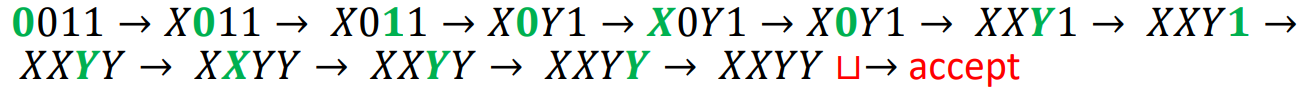
\includegraphics[scale=0.5]{images/turingmachineexampleflow.PNG}
\end{figure}

\noindent
Let $M = (\{q_0, q_1, q_2, q_3, q_{accept}, q_{reject}\}, \{0, 1\}, \{0, 1, X, Y, \sqcup\}, \delta, q_0, q_{accept}, q_{reject})$.\\
At the starting state, cross off the first 0 then move the right:

\[ \delta(q_0, 0) = (q_1, X, R) \] 
\[ \delta(q_0, 1) = (q_{reject}, 1, -) \]

\noindent
Skip over all other 0's and crossed off symbols:

\[ \delta(q_1, 0) = (q_1, 0, R) \]
\[ \delta(q_1, Y) = (q_1, Y, R) \]
\[ \delta(q_1, \sqcup) = (q_{reject}, \sqcup, -) \]

\noindent
When we find the first 1, cross it off and go back:

\[ \delta(q_1, 1) = (q_2, Y, L) \]

\noindent
Skip over all other Y's and 0's:

\[ \delta(q_2, Y) = (q_2, Y, L) \]
\[ \delta(q_2, 0) = (q_2, 0, L) \]

\noindent
When we find an X, go back to the right again:

\[ \delta(q_2, X) = (q_3, X, R) \]

\noindent
If we find another 0, we know we have to go back at least one more time:

\[ \delta(q_3, 0) = (q_1, X, R) \]

\noindent
Skip any Y symbols:

\[ \delta(q_3, Y) = (q_3, Y, R) \]

\noindent
If we reach the end of the string, we know the string is accepted

\[ \delta(q_3, \sqcup) = (q_{accept}, \sqcup, -) \]

\noindent
If we find another 1 symbol, the string is rejected:

\[ \delta(q_3, 1) = (q_{reject}, 1, -) \]

\newpage
\noindent
A Turing machine that \textbf{decides} palindromes:

\begin{figure}[h]
    \centering
    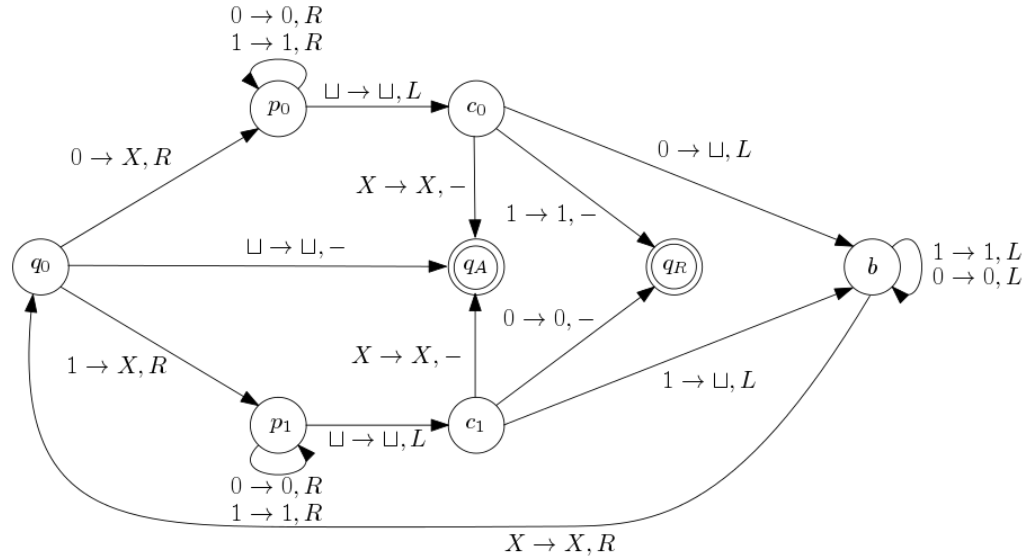
\includegraphics[scale=0.65]{images/turingmachinepalindrome.PNG}
\end{figure}

\noindent
A Turing machine that, given a string $w \in \{0, 1\}^*$, increases $w$ by 1:

\begin{figure}[h]
    \centering
    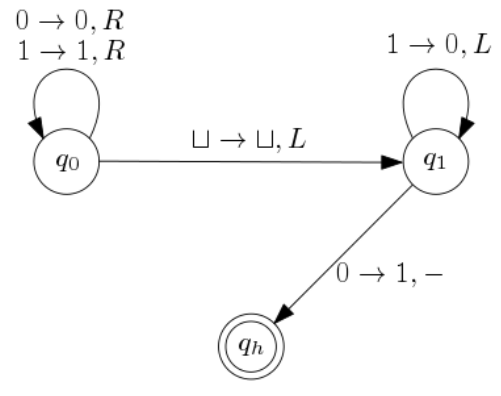
\includegraphics[scale=0.65]{images/turingmachineplusone.PNG}
\end{figure}

\noindent
A Turing machine that, given a string $w \in \{0, 1\}^*$, decreases $w$ by 1:

\begin{figure}[h!]
    \centering
    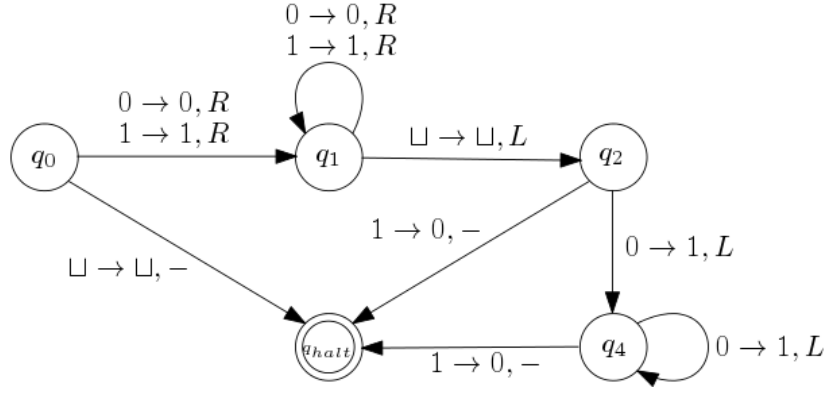
\includegraphics[scale=0.65]{images/turingmachineminusone.PNG}
\end{figure}

%
% Lecture 8
%
\newpage
\section*{Lecture 8 - Variants of Turing Machines}

\subsection*{Multi-tape Turing Machines}
A special Turing machine with multiple tapes.
Each tape has its own cursor for reading and writing.
The input appears on tape 1, the other tapes start all blank.

\begin{figure}[h]
    \centering
    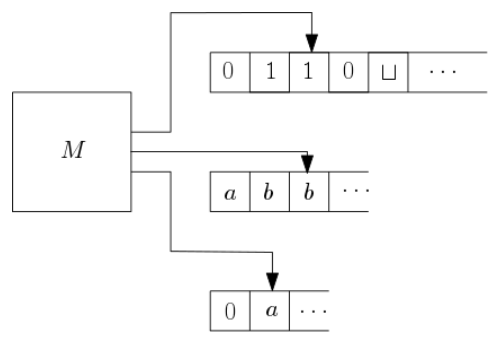
\includegraphics[scale=0.6]{images/multitapeturingmachine.PNG}
\end{figure}

\noindent
A multi-tape Turing machine has transfer function:

\[ \delta: Q \times \Gamma^k \rightarrow Q \times \Gamma^k \times \{L, R, -\}^k \]

\noindent
For example $\delta(q, \sigma_1, \sigma_2, \sigma_3) = (p, \sigma_1^\prime, \sigma_2^\prime, \sigma_3^\prime, L, R, R)$.
"At state $q$ and reading $\sigma_1$ on tape 1, $\sigma_2$ on tape 2 and $\sigma_3$ on tape 3: go to state $p$, change $\sigma_i$ to $\sigma_i^\prime$, move the cursor of the first tape to the left, move the cursor of the second tape to the right and move the cursor of the third tape to the right":

\begin{figure}[h]
    \centering
    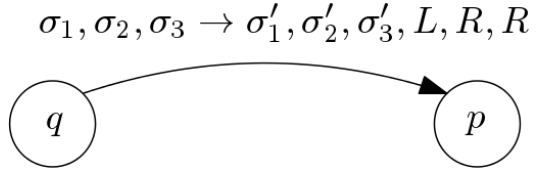
\includegraphics[scale=0.5]{images/multitapevisual.PNG}
\end{figure}

\noindent
An example of a task that is significantly easier with multiple tapes is determining if a string is a palindrome.
With two tapes, you can copy the input to the second tape, move the second cursor to the end of the string, move the first cursor forwards and the second cursor backwards and check if they have the same symbols:

\begin{figure}[h!]
    \centering
    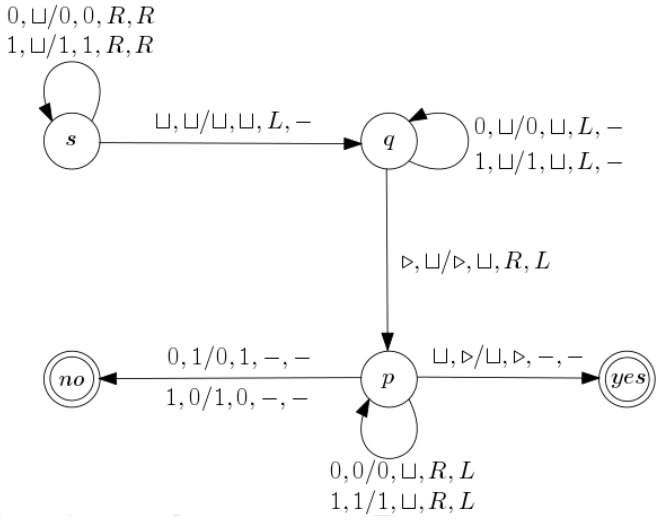
\includegraphics[scale=0.6]{images/multitapepalindrome.PNG}
\end{figure}

\newpage
\noindent
The multi-tape Turing machine can decide if a string is a palindrome in linear ($O(n)$) time:

\begin{itemize}
    \item $n + 1$ steps to copy the input string to the second tape.
    \item $n + 1$ steps to move the first cursor back to the start of the tape.
    \item $n + 1$ steps (at most) to compare the two tapes.\\$---\text{ }+$\\$3n + 1$
\end{itemize}

\noindent
The standard Turing machine takes quadratic time ($O(n^2)$).

\subsection*{From Multi-tape to Single-tape}
Any language recognized / decided by a multi-tape Turing machine can also be recognized / decided by a single-tape Turing machine:

\begin{figure}[h]
    \centering
    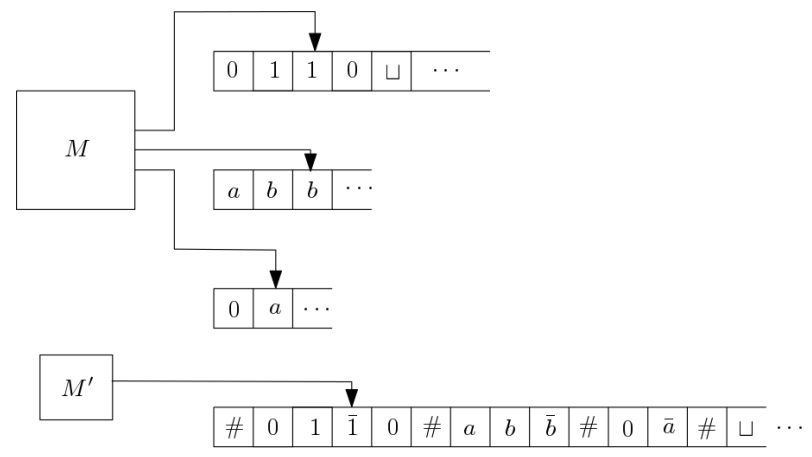
\includegraphics[scale=0.6]{images/multitapetosingletape.PNG}
\end{figure}

\noindent
Specify the concatenation of $k$ different tapes with a special symbol (e.g. $\#$).
Remember the position of each cursor with special symbols:

\[ \# \sigma_1 \overline{\sigma_2} \sigma_3 \# \sigma_4 \overline{\sigma_5} \sigma_6 \# \sigma_7 \overline{\sigma_8} \sigma_9 \# \]

\noindent
This 'simulation' of a multi-tape Turing machine takes $k^2 f(n)^2$ time, where $k$ is the number of tapes and $f(n)$ is the time taken by the multi-tape Turing machine.

\subsection*{Non-deterministic Turing Machines}
A non-deterministic Turing machine is a Turing machine with a \textbf{transition relation} instead of a transition function:

\[ \Delta: Q \times \Gamma \rightarrow 2^{Q \times \Gamma \times \{L, R, -\}} \]

\noindent
For example, $\Delta(q, a) = \{(q, a, L), (p, b, R), (p, b, L)\}$.

\newpage
\noindent
Let $M = (Q, \Sigma, \Gamma, \Delta, q_0, q_{accept}, q_{reject})$ be a non-deterministic Turing machine.
A \textbf{configuration} is a pair $(q, w\underline{a}u)$, where:

\begin{itemize}
    \item $q \in Q$ is the current state of $M$.
    \item $a \in \Gamma$ is the symbol the cursor is currently pointing at.
    \item $w, u \in \Gamma^*$ is the content of the tape to the left and the right of the cursor.
\end{itemize}

\noindent
A configuration $(q, w\underline{a}bu)$ yields in one step the configuration $(q^\prime, wc\underline{b}u)$ if there exists a rule $(q^\prime, c, R) \in \Delta(q, a)$.
This can be denoted by $(q, w\underline{a}bu) \rightarrow (q^\prime, wc\underline{b}u)$ or $(q, w\underline{a}bu) \vdash (q^\prime, wc\underline{b}u)$.
Denote by $\rightarrow^*$ or $\vdash^*$ the reflexive and transitive closure of $\rightarrow$ or $\vdash$, which denotes that a state can be reached in zero or more steps.

\noindent
\\
M \textbf{accepts} string $w \in \Sigma^*$ iff there exists a computation $(q_0, w) \rightarrow^* (q_{accept}, w^\prime)$.\\
M \textbf{recognizes} the language $L \subseteq \Sigma^*$ if $M$ accepts every $w \in L$ (if $w \notin L$ then $M$ rejects or loops forever).\\
M \textbf{decides} the language $L \subseteq \Sigma^*$ iff $M$ accepts every $w \in L$, and rejects every $w \notin L$ (i.e. there exists a computation $(q_0, w) \rightarrow^* (q_{reject}, w^\prime)$).

\noindent
\\
If language $L$ is decided by a non-deterministic Turing machine in time $O(f(n))$, then $L$ is also decided by a \textbf{3-tape} Turing machine in time $O(c^{f(n)})$, where $c$ is the \textit{degree of non-determinism}.
The idea is to try all possible non-deterministic choices (if the 3-tape Turing machine ever finds an accepting state, it also accepts).
This can be imagined as visiting the entire non-deterministic computation tree of the Turing machine in a BFS manner.
The Turing machine uses 3 tapes:

\begin{itemize}
    \item On the first tape, it stores the input $w$ and never changes it.
    \item On the second tape, it simulates the non-deterministic Turing machine on $w$.
    \item On the third tape, it stores the computational path of the non-deterministic Turing machine as a string $\in \Sigma^\prime$. If this string is not a valid computation or does not reach an accepting state, then the third tape is cleared and the next computational path will be tried (in BFS manner).
\end{itemize}

\subsection*{Church-Turing Thesis}
The \textbf{Church-Turing Thesis} says that any real-world (i.e. involving natural numbers) computation can be converted into an equivalent computation involving a Turing machine.

\begin{itemize}
    \item Any proposed model of computation is equivalent to or weaker than Turing machines.
    \item Non-existence of a (good) algorithm in the Turing machine model of computation, means there doesn't exist one at all.
    \item If an algorithm is 'efficient' in one model, it is also 'efficient' in the Turing machine model.
\end{itemize}

\noindent
Turing machines capture the notion of \textbf{"what is computable?"}.
This means from now on we can be more 'high-level' with our Turing machines.
e.g. "if $x$ is a palindrome, accept".

%
% Lecture 9
%
\newpage
\section*{Lecture 9 - Decidability}
A problem is \textbf{decidable} if there is an algorithm (i.e. Turing machine) that decides it.
Examples of problems are:

\begin{itemize}
    \item \textit{Given an undirected graph $G$, is $G$ Eulerian?}
    \item \textit{Given a positive integer $N$, is $N$ prime?}
    \item \textit{Given some function $f(x)$, is $f(x)$ integrable over some domain?}
\end{itemize}

\noindent
Turing machines decide languages, not problems.
We need to represents these objects ($G$, $N$, $f(x)$, etc.) as strings for our Turing machines.
Once we have this representation, the algorithm that decides this problem is the Turing machine that decides the corresponding language.
In general, a representation of an object $O$ is denoted as $\langle O \rangle$.

\noindent
\\
Example:\\
\textbf{Computational problem:} Given $x \in \{0, 1\}^*$, is $x$ a composite number (i.e. not prime)?\\
\textbf{Language problem:} $L = \{w \in \{0, 1\}^* : w \text{ is a binary representation of a composite number}\}$.\\
Let $M$ be a non-deterministic Turing machine on input $w \in \{0, 1\}^*$:

\begin{enumerate}
    \item Choose \textbf{non-deterministically} two positive integers $1 < p, q < w$.
    \item Write down the binary representation of $p$ and $q$ (possibly on a new tape).
    \item Multiply $p$ and $q$ and store the result (possibly on a new tape).
    \item If $p \cdot q = w$, \textbf{accept}. Else, \textbf{reject}.
\end{enumerate}

\noindent
This machine \textbf{decides} $L$.

\noindent
\\
Example:\\
\textbf{Computational problem:} Given a non-directed graph $G$, is $G$ a Hamiltonian graph (i.e. there exists a tour that visits every vertex exactly once)?\\
\textbf{Language problem:} $L = \{G : G \text{ is a Hamiltonian graph}\}$.\\
Let $M$ be a non-deterministic Turing machine on input $G$ with $n$ vertices:

\begin{enumerate}
    \item Choose \textbf{non-deterministically} a permutation of the vertices of $G$ (possibly on a new tape).
    \item Check if $G$ has edges between successive vertices.
    \item If yes, \textbf{accept}. Else, \textbf{reject}.
\end{enumerate}

\noindent
This machine \textbf{decides} $L$.

\newpage
\subsection*{Representation of Objects}
Integers can be represented in binary or any other system.
Graphs can be represented in the adjacency list model, or the adjacency matrix model.
Think of space and time complexity!

\noindent
\\
Example:\\
Let $L = \{\langle G \rangle : G \text{ is a connected undirected graph}\}$.
To decide $L$, we first need to find a way to represent $G$.

\begin{figure}[h]
    \centering
    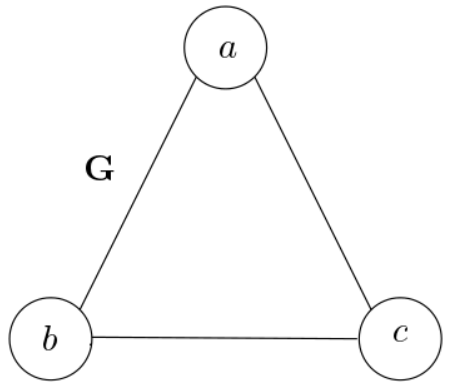
\includegraphics[scale=0.5]{images/graph_representation_example.PNG}
    \caption{This graph can be represented as $\langle G \rangle = (a, b, c), ((a, b), (b, c), (a, c))$.}
\end{figure}

\noindent
Using this representation we can give a high-level description of a Turing machine that decides $L$:

\begin{enumerate}
    \item Select the first vertex of $G$ and mark it.
    \item For every unmarked vertex of $G$, if it is connected to a marked vertex, mark it as well.
    \item Repeat the previous step until no new vertices get marked.
    \item If every vertex is marked, \textbf{accept}. Else, \textbf{reject}.
\end{enumerate}

\newpage
\subsection*{Deciding a DFA}
\textbf{Computational problem:} Given a DFA $D$ and an input string $w$, does $D$ accept $w$?\\
\textbf{Language problem:} $L = \{\langle D, w \rangle : D \text{ is a DFA and accepts string } w\}$.\\
We need to design a Turing machine $M$ such that on input $\langle D, w \rangle$, $M$ accepts iff $D$ accepts $w$:

\begin{enumerate}
    \item Check if $D$ encodes a DFA $(Q, \Sigma, \delta, q_0, F)$, and if $w \in \Sigma^*$.
    \item If no, \textbf{reject}. Else:
    \item Simulate $D$ on $w$ (keep track of $D$'s current state and symbol, update according to $\delta$, etc.).
    \item If the simulation ends on a state $q \in F$, \textbf{accept}. Else, \textbf{reject}.
\end{enumerate}

\noindent
This machine \textbf{decides} $L$.

\subsection*{Deciding an NFA}
$L = \{\langle N, w \rangle : N \text{ is an NFA and accepts string } w\}$.\\
Let $M$ be a Turing machine on input $N$ and $w$:

\begin{enumerate}
    \item Check if $N$ encodes an NFA $(Q, \Sigma, \delta, q_0, F)$, and if $w \in \Sigma^*$.
    \item If no, \textbf{reject}. Else:
    \item Convert $N$ to a DFA $D$ using the standard algorithm.
    \item Use the Turing machine designed for DFA's with input $\langle D, w \rangle$.
    \item If the machine accepts, \textbf{accept}. Else, \textbf{reject}.
\end{enumerate}

\noindent
This machine \textbf{decides} $L$.

\subsection*{Deciding an RE}
$L = \{\langle R, w \rangle : R \text{ is an RE and generates string } w\}$.\\
Let $M$ be a Turing machine on input $R$ and $w$:

\begin{enumerate}
    \item Check if $R$ encodes an RE over some alphabet $\Sigma$, and if $w \in \Sigma^*$.
    \item If no, \textbf{reject}. Else:
    \item Convert $R$ to an NFA $N$ using the standard algorithm.
    \item Use the Turing machine designed for NFA's with input $\langle N, w \rangle$.
    \item If the machine accepts, \textbf{accept}. Else, \textbf{reject}.
\end{enumerate}

\noindent
This machine \textbf{decides} $L$.

%
% Lecture 10
%
\newpage
\section*{Lecture 10 - Undecidability}
Recap non-deterministic Turing machines:
NTM's are equivalent in power to DTM's, but a simulation of them might take up to exponential time.
\textit{"All effective methods of computation are equal to or weaker than the Turing machine"}.
This thesis cannot be proven, but it is widely believed to be true.

\subsection*{Universal Turing Machine}
Is the language $A_{TM} = \{\langle M, x \rangle : M \text{ accepts } x\}$ decidable?
If we want to decide this language we need to simulate a Turing machine, on a Turing machine.
Let $UTM$ be the \textbf{Universal Turing Machine} that, when run on input $\langle M, w \rangle$, where $M$ is a (description of a) Turing machine and $w$ is any string, \textbf{simulates} the computation of $M$ on input $w$.

\[ UTM(\langle M, x \rangle) = M(x) \]

\noindent
If $M$ halts on input $w$ within $O(n)$ steps, then the simulation of $M$ on input $w$ halts within $O(n \log n)$.
This is the most efficient case possible and cannot get any better.

\begin{itemize}
    \item If $M$ \textbf{accepts} $w$, then $UTM$ \textbf{accepts} $\langle M, w \rangle$.
    \item If $M$ \textbf{rejects} $w$, then $UTM$ \textbf{rejects} $\langle M, w \rangle$.
    \item If $M$ \textbf{loops on} $w$, then $UTM$ \textbf{loops on} $\langle M, w \rangle$.
\end{itemize}

\noindent
The Universal Turing Machine looks like this:\\
Assume $M = (Q, \Sigma, \Gamma, \delta, q_0, q_A, q_R)$.
Let $\Sigma = \{1, 2, ... , |\Sigma|\}$, $Q = \{|\Sigma| + 1, ... , |\Sigma| + |Q|\}$ and\\$(L, R, -, q_{halt}, q_A, q_R) = (|\Sigma| + |Q| + 1, ... , |\Sigma| + |Q| + 6)$.
The encoding of $M$ starts with encoding all this information in binary, followed by the encoding of $\delta$ as a sequence of pairs $((q, a), (p, b, D))$, where $q, p \in Q$, $a, b \in \Gamma$ and $D$ is the direction of the cursor.

\begin{figure}[h]
    \centering
    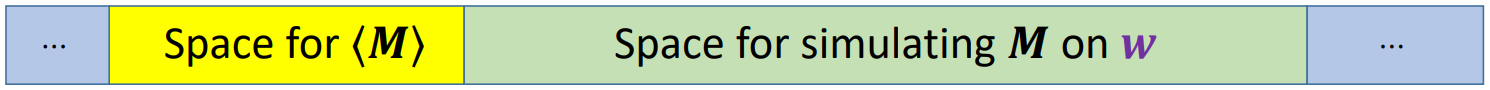
\includegraphics[scale=0.5]{images/utm_tape.PNG}
\end{figure}

\noindent
UTM's are capable of computing everything that could possibly be computable by any conceivable model of computation.
By the Church-Turing thesis: UTM's can simulate any other computation model.

\noindent
\\
For a Turing machine $M$ we can denote the language that is decided by this Turing machine as $L(M) = \{w \in \Sigma^* : M \text{ accepts } w\}$.
We can denote the language decided by the UTM $U$ as $L(U) = \{\langle M, w \rangle : w \in L(M)\}$.

\noindent
\\
Examples:\\
\textbf{Given Turing machine $M$, does $M$ accept the empty string $\epsilon$?}

\[ E_M = \{\langle M \rangle : M \text{ accepts } \epsilon\} \]

\noindent
Does there exist a Turing machine $M^\prime : L(M^\prime) = E_M$?\\
Yes: on input $\langle M \rangle$ construct $\langle M, \epsilon \rangle$.
Feed $\langle M, \epsilon \rangle$ to UTM $U$.
Accept iff $U(\langle M, \epsilon \rangle)$ accepts.

\newpage
\noindent
\textbf{Given Turing machine $M$, does $M$ accept at least one string?}

\[ L_S = \{\langle M \rangle : M \text{ accepts at least one string}\} \]

\noindent
Does there exist a Turing machine $M^\prime : L(M^\prime) = L_S$?\\
We don't know what string it may or may not accept, so we can guess it non-deterministically:\\
On input $\langle M \rangle$ guess $x$ and construct $\langle M, x \rangle$.
Feed $\langle M, x \rangle$ to UTM $U$.
Accept iff $U(\langle M, x \rangle)$ accepts.

\subsection*{The Halting Problem}
Can we \textbf{decide} the language $A_{TM} = \{\langle M, x \rangle : M \text{ is a Turnig machine and accepts string } x\}$?
On the surface this seems like an easy problem.
If $M$ ever enters the accepting state on input $x$, accept.
If $M$ ever enters the rejecting state on input $x$, reject.
But what if $M$ never halts?

\noindent
\\
Let $H$ be a decider for $A_{TM}$.\\
Let $D$ be a Turing machine that, on input $\langle M \rangle$, does the following:

\begin{enumerate}
    \item Run $H$ on input $\langle M, \langle M \rangle \rangle$,
    \item If $H$ accepts $\langle M, \langle M \rangle \rangle$, \textbf{reject}.
    \item If $H$ rejects $\langle M, \langle M \rangle \rangle$, \textbf{accept}.
\end{enumerate}

\noindent
In short, $D(\langle M \rangle) = $ accept if $M$ does not accept $\langle M \rangle$,  $D(\langle M \rangle) = $ reject if $M$ does accept $\langle M \rangle$.\\
What happens when we run $D(\langle D \rangle)$?

\begin{itemize}
    \item $D(\langle D \rangle) = $ \textbf{accept} if $D$ rejects $\langle D \rangle$.
    \item $D(\langle D \rangle) = $ \textbf{reject} if $D$ accepts $\langle D \rangle$.
\end{itemize}

\noindent
$D(\langle D \rangle)$ accepts iff $D$ does not accept $\langle D \rangle$.
This is a contradiction.
Thus, $H$ and $D$ \textit{cannot} exists.
Thus, the language $A_{TM}$ is \textbf{undecidable}.

\noindent
\\
We can use this to prove that other languages are undecidable.
If we assume a decider for a language, then use that decider to solve the halting problem, we can conclude that that language is undecidable.

\noindent
\\
Example:
\[ HALT_{TM} = \{\langle M, w \rangle : M \text{ is a Turing machine and halts on input } w\} \]

\noindent
Assume $R$ decides $HALT_{TM}$.
Using $R$ we can build a Turing machine $S$ that does the following:

\begin{enumerate}
    \item Run $R(\langle M, w \rangle)$,
    \item If $R(\langle M, w \rangle)$ rejects, then \textbf{reject}.
    \item If $R(\langle M, w \rangle)$ accepts, then simulate $M$ on $w$ until it halts, and \textbf{accept} iff $M$ accepts $w$.
\end{enumerate}

\noindent
This machine decides $A_{TM}$, and therefore solves the halting problem.
Thus, the language $HALT_{TM}$ is \textbf{undecidable}.

\newpage
\subsection*{The Emptiness Problem}

\[ E_{TM} = \{\langle M \rangle : M \text{ is a Turing machine and } L(M) = \varnothing\} \]

\noindent
Assume $R$ decides $E_{TM}$.
Using $R$ we can build a Turing machine $S$ that does the following:

\begin{enumerate}
    \item Create a copy of $M$, $M^\prime$, that rejects every string \textbf{except} $w$.
    \item On input $w$, $M^\prime$ behaves exactly the same as $M$.
    \item Use $R$ to determine if $L(M^\prime) = \varnothing$.
    \item If $L(M^\prime) = \varnothing$, then $M$ does not accept $w$.
    \item If $L(M^\prime) \neq \varnothing$, then $M$ does accept $w$.
\end{enumerate}

\noindent
This machine solves the halting problem.
Thus, the language $E_{TM}$ is \textbf{undecidable}.

\subsection*{The Equivalence Problem}

\[ EQ_{TM} = \{\langle M_1, M_2 \rangle : M_1, M_2 \text{ are Turing machines and } L(M_1) = L(M_2)\} \]

\noindent
Assume $R$ decides $EQ_{TM}$.
Using $R$ we can build a Turing machine $S$ that does the following:

\begin{enumerate}
    \item Construct a Turing machine $M_1$ that rejects every input ($L(M_1) = \varnothing$).
    \item Run $R(\langle M, M_1 \rangle)$,
    \item If $R$ accepts $\langle M, M_1 \rangle$, accept.
    \item Else, reject.
\end{enumerate}

\noindent
This machine decides the language $E_{TM}$, which solves the emptiness problem.
Thus, $R$ and $S$ cannot exist.
Thus, the language $EQ_{TM}$ is \textbf{undecidable}.

%
% Lecture 11
%
\newpage
\section*{Lecture 11 - Intro to Complexity Theory}
\textbf{Computational Complexity Theory} focuses on classifying computational problems according to how easy or difficult it is to solve them.
We will mostly focus on \textbf{time complexity}:

\noindent
\\
Given a Turing machine $M$ that \underline{halts on all inputs}, the \textbf{time complexity} of $M$ is a function $f: \mathbb{N} \rightarrow \mathbb{N}$ such that $f(n)$ is the \textit{maximum} number of steps $M$ needs to halt on any input of length $n$.

\subsection*{Complexity Classes}
The \textbf{Time Complexity Class} $TIME(t(n))$ is the set of all languages $L$ for which there exists a Turing machine that decides $L$ in time $t(n)$.
For example:

\begin{itemize}
    \item $L = \{0^n 1^n : n \geq 0\} \in TIME(n^2)$
    \item $L = \{w : w = w^R\} \in TIME(n)$ (with 2-tape Turing machine)
    \item $L = \{\langle n \rangle : n \text{ is a prime number}\} \in TIME(\sqrt{2^{|n|}})$
    \item $L = \{\langle G \rangle : G \text{ is a connected graph}\} \in TIME(|V(G)| + |E(G)|)$
\end{itemize}

\noindent
Keep in mind different models of computation can yield different complexities for the same language (e.g. some language might be able to be decided easier with a multi-tape Turing machine).

\noindent
\\
Similar to $TIME$, there also exist complexity classes for $RESOURCE$, $SPACE$, $RANDOMNESS$, etc. that work in the same way.
Some of the most notable complexity classes include:

\begin{itemize}
    \item $L$: all problems solvable in logarithmic space
    \item $P$: all problems solvable in deterministic-polynomial time
    \item $NP$: all problems solvable in non-deterministic-polynomial time
    \item $PSPACE$: all problems solvable in deterministic-polynomial space
    \item $EXP$: all problems solvable in deterministic-exponential time
    \item $EXPSPACE$: all problems solvable in exponential space    
\end{itemize}

\[ L \subseteq P \subseteq NP \subseteq PSPACE \subseteq NPSPACE \subseteq EXPTIME \subseteq NEXPTIME \]

\[ P = \{L : L \text{ can be decided by a DTM in polynomial time for every input}\} \]
\[ P = \{L : \exists \text{ a DTM } M \text{ such that } L(M) = L \text{ and } M \in TIME(n^k), k \geq 0\} \]

\noindent
\\
(The set of all DTMs that, on input $w$, complete their computation within $O(|w|^k)$ steps, where $k \geq 0$ is a constant independent of $|w|$.)

%
% Lecture 12
%
\newpage
\section*{Lecture 12 - Reductions}
A reduction from problem $A$ to problem $B$ means that if we find an algorithm that can solve problem $B$, we can also use that algorithm to solve problem $A$.
For example: "In order to become a programmer, I need to learn C".
The task of "becoming a programmer" \textbf{reduces} to "learning C".

\noindent
\\
We can also use reductions to show that some problems \textit{can't} be solved:
If we know that an algorithm for problem $A$ cannot exist, then reducing problem $B$ to problem $A$ proves that problem $B$ cannot be solved either.

\begin{figure}[h]
    \centering
    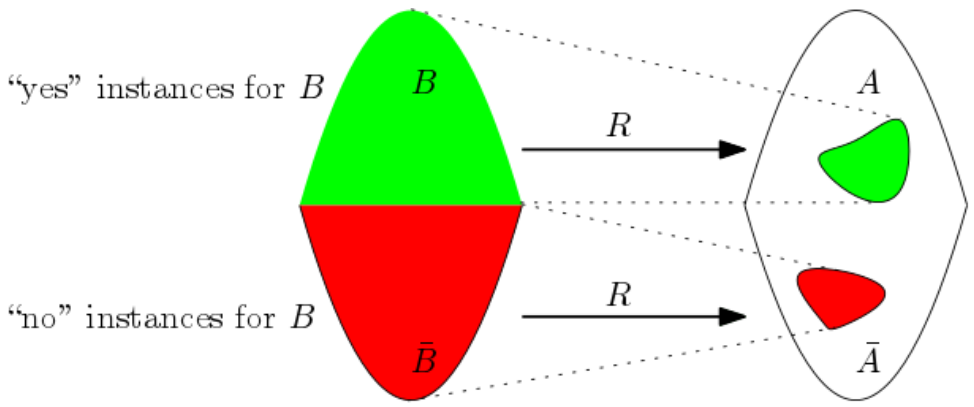
\includegraphics[scale=0.5]{images/reductions.PNG}
    \caption{A reduction maps \textit{yes} instances to \textit{yes} instances and \textit{no} instances to \textit{no} instances.}
\end{figure}

\noindent
How to solve a problem using reductions:

\begin{enumerate}
    \item Let $R$ be a reduction from problem $A$ to problem $B$ ($R$ transforms instances of $A$ to instances of $B$ with the same answer).
    \item Let $M$ be an algorithm for problem $B$: $M$ on input $I_B$ answers correctly whether $I_B$ is a \textit{yes} or \textit{no} instance for problem $A$.
    \item Use $M$ and $R$ to construct an algorithm $N$ that solves problem $A$ as follows: $N$ on input $I_B$ uses $R$ to construct $I_A$, then returns $M(I_A)$.
\end{enumerate}

\begin{figure}[h]
    \centering
    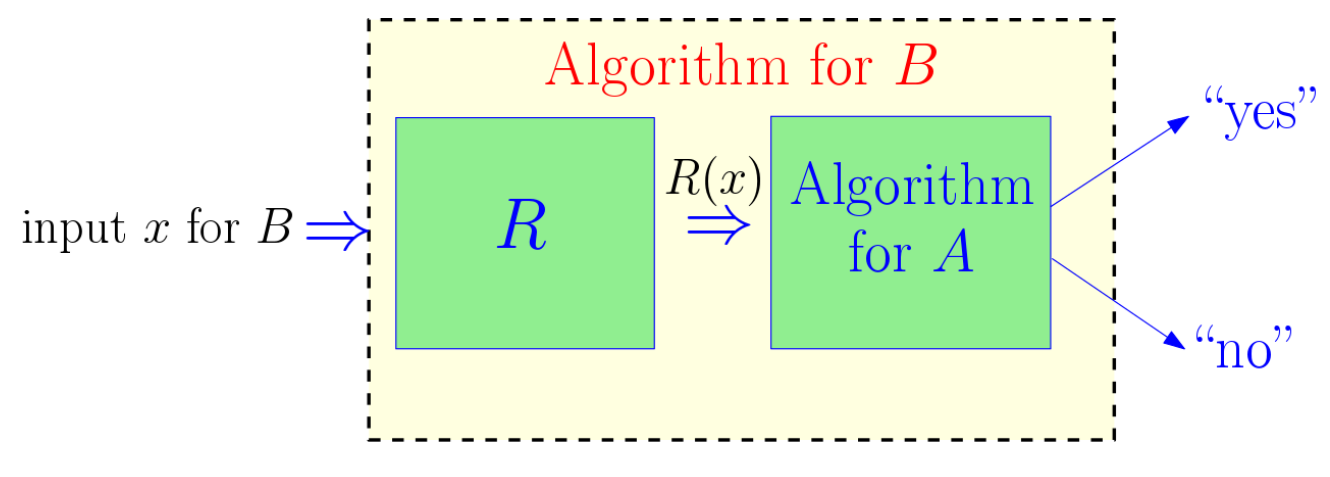
\includegraphics[scale=0.5]{images/reductionalgorithm.PNG}
\end{figure}

\newpage
\subsection*{Comparing Problems}
If $B$ reduces to $A$, we can write $B \leq A$ to denote that $B$ \textbf{is not harder than} $A$, or $A$ \textbf{is at least as hard as} $B$.
Furthermore:

\begin{itemize}
    \item If $B$ reduces to $A$ and $B$ is hard, then $A$ is hard as well.
    \item If $B$ reduces to $A$ and $A$ is easy, then $B$ is easy as well.
\end{itemize}

\noindent
\textit{(Assuming that the reduction from $B$ to $A$ is not incredibly hard to compute)}

\noindent
\\
Examples:\\
\textbf{Given a simple non-directed graph $G$, can we decide if $G$ is bipartite?}

\noindent
\\
$G$ is bipartite iff it does not have any odd-length cycles.
This means that if we had an algorithm $C$ to tell us if a graph has any odd-length cycles, we could use it to solve this problem as well:

\begin{enumerate}
    \item Run $C(\langle G \rangle)$.
    \item Iff $C(\langle G \rangle)$ returns \textit{yes}, then $G$ is not bipartite.
\end{enumerate}
\[ \text{bipartiteness } \leq \text{ decide odd-cycles} \]

\noindent
This reduction is called the \textbf{identity algorithm}.
If we give $\langle G \rangle$ as input, we pass it as input to another problem and use that answer to solve the initial problem.

\noindent
\\
Given two problems:\\
\textbf{Given a simple non-directed graph $G$ and a positive integer $k$, does $G$ have an independent set $V_1$ of size $\geq k$?}\\
\textbf{Given a simple non-directed graph $G$ and a positive integer $k$, does $G$ have a clique $V_2$ of size $\geq k$?}

\noindent
\\
An instance of the independent set problem $\langle G, k \rangle$ is a representation of a graph $G$ and an integer $k$.
Remember how a reduction $R$ from the independent set problem to the clique problem is an algorithm that transforms instances $\langle G, k \rangle$ to instances $\langle G^\prime, k^\prime \rangle$ such that:

\begin{itemize}
    \item If $\langle G^\prime, k^\prime \rangle$ is a \textit{yes} instance for the clique problem, $\langle G, k \rangle$ is a \textit{yes} instance for the independent set problem.
    \item If $\langle G^\prime, k^\prime \rangle$ is a \textit{no} instance for the clique problem, $\langle G, k \rangle$ is a \textit{no} instance for the independent set problem.
\end{itemize}

\noindent
To solve our problem, take $R$ on input $\langle G, k \rangle$ outputs $\langle \bar{G}, k \rangle$ (where $\bar{G}$ is the complement of $G$).
\textit{(proof redacted)}

\noindent
\\
This tells us that the independent set problem is $\leq$ the clique problem, but also that the clique problem is $\leq$ the independent set problem.
Thus, we have proven that the independent set problem and the clique problem are identical problems (in terms of complexity).

%
% Lecture 13
%
\newpage
\section*{Lecture 13 - Polynomial Time}
\[ P = \{L : L \text{ can be decided by a DTM in polynomial time for every input}\} \]

\[ P = \bigcup_i TIME(n^i), \text{  } i \geq 1 \]

\noindent
$P$ corresponds to the concept of \textbf{efficient} computation.
We can also view the complexity class $P$ as a collection of problems which can be solved in polynomial time:

\[ P = \{\text{all problems for which a polynomial time algorithm (TM) exists}\} \]

\noindent
How to prove that a problem belongs to $P$:

\begin{itemize}
    \item \textbf{Direct Proof:} construct an algorithm that runs in $O(|w|^k)$ on every input $w$.
    \item \textbf{Proof using Closure Properties:} proof that the language of the problem can be formed using transformations of other languages known to be in $P$.
    \item \textbf{Proof using Reductions:} reduce the problem $B$ to a problem $A$ already known to be in $P$ (make sure the reduction itself can be done in polynomial time as well!).
\end{itemize}

\noindent
A problem $B$ reduces to problem $A$ ($B \leq A$) if there is an algorithm $R$ that transforms instances $x$ of $B$ to instances $R(x)$ of $A$ such that:

\[ x \in B \Leftrightarrow R(x) \in A \]

\noindent
If $R$ runs in polynomial time w.r.t. $|x|$ then $R$ is a \textbf{polynomial-time reduction}:

\[ B \leq_p A \]

\begin{itemize}
    \item If $B \leq_p A$ and $A$ is \textit{easy} (i.e. $A \in P$), then $B$ is also \textit{easy} ($B \in P$).
    \item If $B \leq_p A$ and $B$ is \textit{hard}, then $A$ is also \textit{hard} (if it wouldn't be hard, then $B$ would be easy).
\end{itemize}

\subsection*{Beyond Polynomial Time}
Given $\langle G \rangle$, the description of a simple, non-directed graph $G$, is there a path that visits every vertex of $G$ exactly once? (\textbf{Hamiltonian Path Problem})

\noindent
\\
Currently the fastest algorithms we know solve this in $O(n^2 2^n)$ or $O(1.657^n)$, which means\\$\text{HamiltonianPath} \notin TIME(n^k)$.

\noindent
\\
Alternative strategy: guess path $p$ non-deterministically, then check if $p$ is Hamiltonian (linear time).
This means $\text{HamiltonianPath} \in NTIME(n)$, where $NTIME$ means \textbf{non-deterministic time}.

\newpage
\subsection*{Non-Deterministic Computation}
Let $N$ be a \textbf{non-deterministic} Turing machine that halts on all inputs.
The time complexity of $N$ is a function $f: N \rightarrow N$ such that $N$ halts on all inputs of length $n$ within at most $f(n)$ steps.
There can be multiple functions $f$ that provide an upper bound on the number of steps, you should choose the function with the lowest upper bound (\textbf{supremum}).
$f(n)$ is the maximum length of any branch of the non-deterministic computational tree.

\noindent
\\
The complexity class $NTIME(f(n))$ is the set of all non-deterministic Turing machines that halt on all inputs of length $n$ within at most $f(n)$ steps.
\[ NTIME(f(n)) = \{L : L \text{ is decided by a non-deterministic Turing machine operating in } O(f(n))\} \]

\noindent
\textbf{Theorem:} every deterministic computation is also a non-deterministic computation, and every non-deterministic computation can be simulated in exponential time:

\[ TIME(f(n)) \subseteq NTIME(f(n)) \subseteq TIME(2^{f(n)}) \]

\subsection*{The NP Class}

\[ NP = \bigcup_i NTIME(n^i), \text{  } i \geq 1 \]

\noindent
$NP$ stands for \textbf{non-deterministic polynomial}.
$NP$ contains all decision problems for which we can \textbf{guess} (non-deterministically) a solution in polynomial time and then \textbf{verify} this solution again in polynomial time.

\noindent
\\
$P$ is the set of problems for which we can easily \textit{find} the solution.\\
$NP$ is the set of problems for which, once we have the solution, we can easily \textit{verify} it.

\noindent
\\
Example: take a lock; finding the password to the lock is hard ($\notin P$), but once we have the password it is very easy to verify ($\in NP$).

%
% Lecture 14
%
\newpage
\section*{Lecture 14 - NP-Completeness}
$NP$ contains all languages $L$ for which the statement $w \in L$ has a short, easily verifiable proof ($O(|w|^k)$).
This short proof is called the \textbf{certificate}.
If $w \in L$ and $L \in NP$ then there must be some short information that can easily (polynomial time) convince everyone that $w \in L$.

\noindent
\\
Example: Does a Sudoku have a solution?

\begin{enumerate}
    \item Non-deterministically guess the solution. ($n^2$)
    \item Deterministically verify the solution ($n^2$)
    \item If yes, accept. Else, reject.
\end{enumerate}

\noindent
Sudoku $\in NP$.

\noindent
\\
A language $L \in NP$ iff there exists a \textbf{deterministic} polynomial time Turing machine $V$ such that:

\[ L = \{x : \exists y \in \Sigma^*, |y| = |x|^k \text{ and } V(x, y) \text{ accepts}\} \]

\noindent
$V$ is called a \textbf{verifier}, it verifies $x \in L$ with the help of $y$.\\
$y$ is the \textbf{certificate} that proves that $x$ is a \textit{yes} instance (i.e. $x \in L$).

\noindent
\\
We say that a problem $A$ is \textbf{NP-Complete}, if $A \in NP$ and all problems in $NP$ polynomially reduce to $A$:

\[ \forall B \in NP \text{, } B \leq_p A \]
\[ \text{"$A$ is at least as hard as any other problem in $NP$"} \]

\noindent
\\
If all problems in $NP$ polynomially reduce to $A$, but $A$ is not (known to be) in $NP$, then we say $A$ is \textbf{NP-Hard}.

\begin{figure}[h]
    \centering
    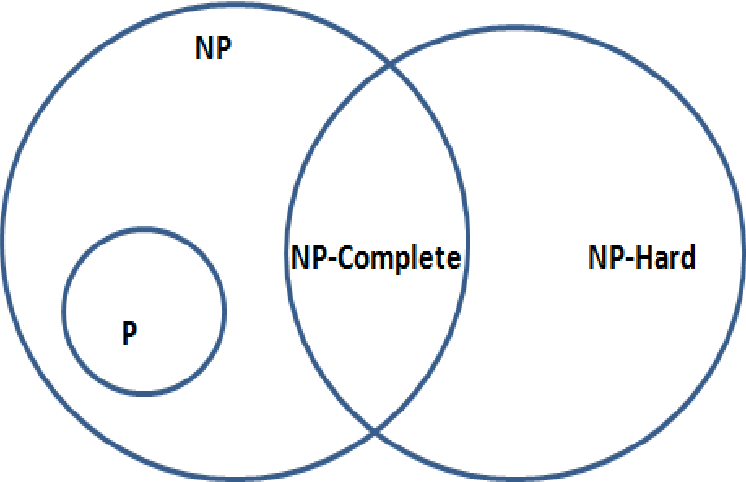
\includegraphics[scale=0.35]{images/npvenndiagram.png}
\end{figure}

\newpage
\noindent
If we want to prove that a problem $B$ is \textbf{NP-Complete}, we have to prove two things:

\begin{enumerate}
    \item $B \in NP$
    \item Some already-known NP-Complete problem $C$ reduces in poly-time to $B$: $C \leq_p B$.
\end{enumerate}

\noindent
Be careful not to reduce $B$ to $C$!
Since $C$ is already known to be NP-Complete, we know all problems in $NP$ (including $B$) reduce to it.
Some problems that are known to be NP-Complete:

\subsection*{The Satisfiability Problem}
Consider a set $V$ of boolean variables $x_1, x_2, ... , x_n$:

\begin{itemize}
    \item \textbf{Literal:} a boolean value ($x_i$), or its negation ($\neg x_i$).
    \item \textbf{Clause:} a disjuction (OR) of literals (e.g. $x_1 \lor x_2 \lor \neg x_3$).
    \item \textbf{Formula:} a conjuction (AND) of clauses (e.g. $(x_1 \lor x_2) \land (\neg x_2 \lor x_3)$).
\end{itemize}

\noindent
A boolean formula applying to these conventions is called a formula in \textbf{Conjuctive Normal Form (CNF)}.
Example: $(x_1 \lor x_2) \land (\neg x_2 \lor x_3)$ is written in CNF, while $\neg (B \lor C)$ and $(A \land B) \lor C$ are not.

\noindent
\\
\textbf{Satisfiability Problem}, or \textbf{SAT-Problem}: Given a boolean formula $\Phi$ in CNF, is there a variable assignment $V \rightarrow \{\text{true},\text{false}\}$ such that $\Phi$ evaluates to true? (is $\Phi$ satisfiable?)

\noindent
\\
Theorem: $SAT \in NTIME(n)$, where $n = \langle \Phi \rangle = \#\text{clauses} + \#\text{literals}$.\\
Proof: We will describe a non-deterministic Turing machine $M$ with input $\langle \Phi \rangle$ that decides $SAT$:

\begin{enumerate}
    \item Check if $\langle \Phi \rangle$ is in CNF, reject if not.
    \item For each variable $x_i \in V(\Phi)$, non-deterministically guess its value (true or false).
    \item Substitute the truth value of $x_i$ in $\Phi$.
    \item Accept if the assignment satisfies $\Phi$, reject otherwise.
\end{enumerate}

\noindent
This Turing machine decides the $SAT$ problem.

\noindent
\\
\textbf{Cook-Levin Theorem:} The $SAT$ problem is NP-Complete.
This is done by building a poly-time reduction from an arbitrary problem $B \in NP$, that turns the input string $w$ into a CNF formula $\Phi$.

\subsection*{3SAT Problem}
\[ 3SAT = \{ \Phi : \Phi \text{ is a satisfiable, boolean CNF formula such that each clause has at most 3 literals} \} \]

\noindent
If we want to prove that $3SAT$ is NP-Complete, we first have to prove that $3SAT \in NP$:

\noindent
\\
Given $\langle \Phi \rangle$, check if it is in CNF and if every clause has at most 3 literals.
Non-deterministically guess a truth assignment, then check if this assignment is correct.

\newpage
\noindent
Next, we need to prove that $SAT$ reduces to $3SAT$ in poly-time ($SAT \leq_p 3SAT$):

\noindent
\\
Given $\Phi$, an input instance of $SAT$, we will construct an input instance for $3SAT$ $\Phi^\prime$ such that:

\begin{itemize}
    \item $\Phi^\prime$ is satisfiable iff $\Phi$ is.
    \item We can construct $\Phi^\prime$ in polynomial time compared to $|\langle \Phi \rangle|$.
\end{itemize}

\noindent
If $\Phi$ has a clause that is longer than 3 literals, we will split it up into several clauses with a maximum length of 3.
For example, if $\Phi$ has the clause $(l_1 \lor l_2 \lor l_3 \lor l_4)$, $\Phi^\prime$ will have the clause $(l_1 \lor l_2 \lor u_1) \land (\neg u_1 \lor l_3 \lor l_4)$.
Because the logical meaning of $\Phi$ isn't changed by this, we can conclude $\Phi \Leftrightarrow \Phi^\prime$.

\subsection*{Independent Set Problem}
\[ IndSet = \{\langle G, k \rangle : G \text{ has an independent set of size } k\} \]

\noindent
Proof that $IndSet \in NP$:

\noindent
\\
Given $\langle G, k \rangle$, non-deterministically guess a set of vertices of size $k$, then check if this set is a valid independent set.

\noindent
\\
Proof that $3SAT \leq_p Indset$:

\noindent
\\
For each clause in $\Phi$, create a clique of nodes where each node represents a literal in the clause.
After making cliques for every clause, connect all nodes that have an opposite literal (i.e. connect any $(x)$ nodes with $(\neg x)$ nodes).
$\Phi$ is satisfiable iff this graph has an independent set of size $k$ (where $k$ is the number of clauses in $\Phi$).

\noindent
\\
Corollary to this proof, the \textbf{k-Clique} and \textbf{k-VertexCover} problems are also NP-Complete:

\[ SAT \leq_p 3SAT \leq_p IndSet \leq_p Clique \leq_p VertexCover \]

\subsection*{P vs NP}
$P = \{L : \text{there exists a poly-time deterministic Turing machine that decides } L\}$\\
$NP = \{L : \text{there exists a poly-time non-deterministic Turing machine that decides } L\}$

\noindent
\\
If $P = NP$, then that means if a proof can be \textit{verified} quickly, it can also be \textit{found} quickly.
Most scientists believe $P \neq NP$, as that is where the current evidence is pointing to.
However this has not yet been formally proven.
Some scientists believe that the reason $P \neq NP$ is so difficult to (dis)prove, is because $P \neq NP$.

\noindent
\\
If one NP-Complete problem is found to have a poly-time solution, then that proves $P = NP$ (through the fact that all NP problems can be reduced to an NP-Complete problem).

\end{document}
